%!TEX program = xelatex
% 完整编译: xelatex -> bibtex -> xelatex*2
\documentclass[11pt,a4paper]{elegantpaper}
% \usepackage{etex}
\usepackage{xeCJK}
\usepackage{CJK}
\setCJKmainfont{STSong}
\setmainfont{Times New Roman}
\newcommand{\tm}{\fontspec{Times New Roman}}
% \newCJKfontfamily{\STSong}[AutoFakeBold={3.17}]{STSong}
\newCJKfontfamily{\heiti}[AutoFakeBold={3.17}]{SimHei}
\newCJKfontfamily{\fangsong}[AutoFakeBold = {3.17}]{FangSong_GB2312} 
\newCJKfontfamily{\huawenxingkai}[AutoFakeBold={2.17}]{STXingkai}
% \documentclass{cn}{elegantpaper}
\usepackage{fancyhdr}
\usepackage{geometry}
\usepackage{multicol}    % 正文双栏
\usepackage{abstract}    % 2栏文档,一栏摘要及关键字宏包

\usepackage{ulem}
\usepackage{amsmath}
\usepackage{graphicx}
\usepackage{caption}
\usepackage{float} %设置图片浮动位置的宏包
\usepackage{subfigure} %插入多图时用子图显示的宏包
\usepackage{amssymb}
\usepackage{listings}

\lstset{
	breaklines=true,  %代码过长则换行
	keywordstyle= \color{blue},%关键字颜色
}

\setlength{\topmargin}{-1cm}
\setlength{\oddsidemargin}{-0.9cm}  % 3.17cm - 1 inch
\setlength{\evensidemargin}{\oddsidemargin}
\setlength{\headheight}{12pt}
\setlength{\headsep}{12pt}
\setlength{\textwidth}{17.00cm}
\setlength{\textheight}{24.62cm}    % 24.62
%CDSS(VScode \LaTeX  Test)\\
\title{\Huge{\textbf{\STSong{脱丁烷塔软测量实验报告}}}\\
\LARGE{\textbf{\STSong{Project Report of Soft Sensing for Debutanizers \\ \quad }}}\\ 

\includegraphics[width=3cm]{images/1024px-Zhejiang_University_Logo.png}}
% \centering
% Zhejiang_University_Logo
\author{\normalsize 王子非\footnote{王子非:自动化控制1903,3190105833},刘可佳\footnote{刘可佳:自动化电气1902,3190102982},  李浩东\footnote{李浩东:自动化控制1904,3190104890}  \\ \small Zifei WANG, Kejia LIU,  Haodong LI}
\institute{\normalsize 浙江大学控制科学与工程学院\\ 
\small{College of Control Science and Engineering, Zhejiang University} \\ }

\date{2022年01月14日\quad \today \\ }

\renewcommand{\headrulewidth}{0.4pt}
\usepackage{setspace}
\onehalfspacing%1.5倍行距
\addtolength{\parskip}{.4em}%段间距

\newcommand{\makeheadrule}{%
\makebox[0pt][l]{\rule[0.55\baselineskip]{\headwidth}{0.4pt}}%
\rule[0.7\baselineskip]{\headwidth}{0.4pt}}
\renewcommand{\headrule}{%
{\if@fancyplain\let\headrulewidth\plainheadrulewidth\fi
\makeheadrule}}

% 页眉页脚
\fancypagestyle{plain}{
\renewcommand{\footrulewidth}{0pt}
\fancyhf{}
\lhead{冬~学~期~课~程~报~告\quad \quad \\
\scriptsize{2022~~年~~1~~月}}
\chead{\centering{数~据~驱~动~建~模~与~应~用\\
\scriptsize{\textbf{Data Driven Modeling and Applications}}}}
\rhead{Winter Semester, Course Paper\\
\scriptsize{January, 2022}}
\cfoot{\thepage}}

% \lhead{软件复杂度与bug对软件质量的影响}
% \chead{}
% \rhead{The impact of software complexity and bugs on software quality}
% R,C,L分别代表左中右,O,E代表奇偶页
\pagestyle{fancy}
% \lhead{\rightmark}
% \rhead{\rightmark}
\chead{脱丁烷塔软测量实验报告}
\cfoot{\thepage}
\usepackage{abstract}
\newCJKfontfamily{\STSong}[AutoFakeBold={1.585}]{STSong}

\begin{document}

\newcommand{\supercite}[1]{\textsuperscript{\cite{#1}}}
\renewcommand{\thefootnote}{\Roman{footnote}}

% \begin{figure}[H]
%   \centering
%   
\includegraphics{images/1024px-Zhejiang_University_Logo.png}
% \end{figure}

\maketitle

\renewcommand{\abstractname}{\textbf{\STSong{摘\quad 要}}\\}
\begin{abstract}
\textbf{\quad\quad}本次项目中,我组首先针对数据中的不同维度进行数据分析,之后再分析的基础上进行合适的预处理,之后进行模型的搭建与检验评估。
我们使用了OLS、PLS、随机森林、SVM、BP神经网络、DNN、CNN、LSTM、RNN等方法进行脱丁烷塔软测量的温度预测,最终使用LSTM模型跑出了0.087908的成绩,位列第一。
\\ \\ 
\textbf{\STSong{关键词}}:回归,LSTM\\ 
\end{abstract}

\renewcommand{\abstractname}{\textbf{\STSong{Abstract}}\\}
\begin{center}
\textbf{\STSong{Abstract}}
\end{center}
% \newcommand{\abstracttextfont}{\}
\begin{quote}
  In this project, our group firstly analyzed the data vary on different dimensions, and 
  then conducted appropriate preprocessing operations based on the analysis. After that, 
  we performed model construction, training, inspection, and evaluation.
  We used OLS, PLS, random forest, SVM, BP neural network, DNN, CNN, LSTM, RNN and other methods 
  to predict the temperature of the soft-sensor of the butanizer, and finally used the LSTM model 
  to get a score of 0.087908, ranking No. 1.
\keywords{Key Words: Regression, LSTM\\}
\end{quote}

\begin{multicols}{2}
% \begin{twocolumn}
\section{引言}

\subsection{项目背景}

随着现代工业过程对质量控制、可靠性等要求的不断提高,质量相关的过程变量进行实时监测和控制变得更加重要。然而在复杂的工业生产过程中,由于工艺和条件的限制,存在许多难以直接测量的变量。这些变量虽然可以用在线分析仪进行测量,但是由于在线分析仪表(传感器)不仅价格昂贵、维护保养复杂,而且由于分析仪表滞后大等原因,最终将导致控制质量的性能下降,难以满足生产要求。还有部分产品质量目前无法测量(例如某些成分的浓度)。

为了解决上述问题,软测量技术作为具有广阔发展前景的新兴技术应运而生。软测量建模代替了传统的传感器,其核心是对于一些难以测量的重要变量(主导变量),选择另外一些容易测量的变量(辅助变量)通过构建数学模型,以实现对主导变量的最佳估计。目前常用的软测量建模方法有主元回归(PCR)、偏最小二乘回归(PLS)、支持向量回归(SVR)、人工神经网络(ANN)等。

在实际过程中,软测量模型投入运行后,由于催化剂老化、设备老化、原料变化、产品质量要求改变等过程时变特性以及建模样本的不完备性,随着时间的推移,离线建立的软测量模型预测精度会下降,出现“模型老化”现象,导致模型的输出估计值出现较大的偏差,不再适应当前的工况特性。因此需要对软测量模型进行自适应更新,根据在线样本数据不断修正模型参数以适应过程时变特性。

目前常用的对模型进行更新的方法有滑动窗方法和递归方法,能够有效处理慢时变过程,对于过程突变或者变化相对频繁的过程,这类方法效果并不理想。为了解决这个问题,国外学者Cheng(2005)提出基于即时学习(JITL)的局部建模方法用于非线性过程的建模。该方法对于待预测的样本,在历史数据中找出与其最相似的若干个样本建立局部模型,通过局部模型进行在线预测输出。JITL方法既能解决过程时变问题,又能解决过程非线性问题,主要特征有以下几个方面

\begin{enumerate}
  \item 局部建模针对当前样本建立
  \item 采用对应的局部模型计算当前样本的输出预测值
  \item 局部模型随着当前样本进行实时更新
\end{enumerate}

似度准则的选取是JITL建模的核心部分,对于局部模型的预测精度至关重要。

\subsection{问题描述}

脱丁烷塔是脱硫和石脑油分馏装置的一部分(如图1)。在脱丁烷塔中,C3(丙烷)和C4(丁烷)作为杂质从石脑油馏分中除去。脱丁烷塔详细示意图如图2所示。

\begin{figure}[H]
  \centering
  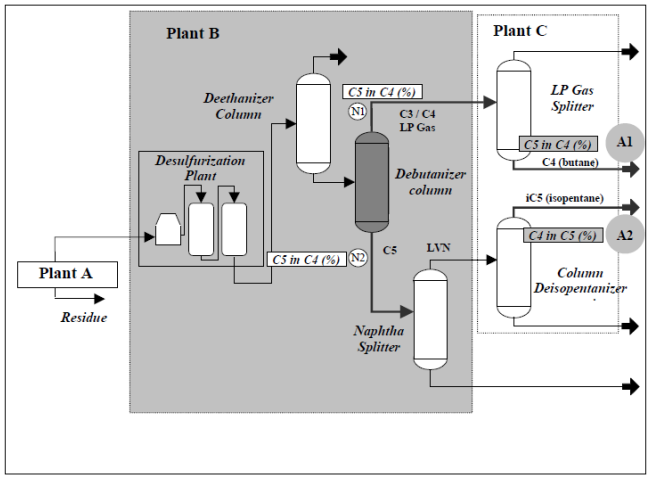
\includegraphics[width=0.5\textwidth]{images/TT.png}
  \caption{脱丁烷塔和其他相连过程示意图} 
\end{figure}

\begin{figure}[H]
  \centering
  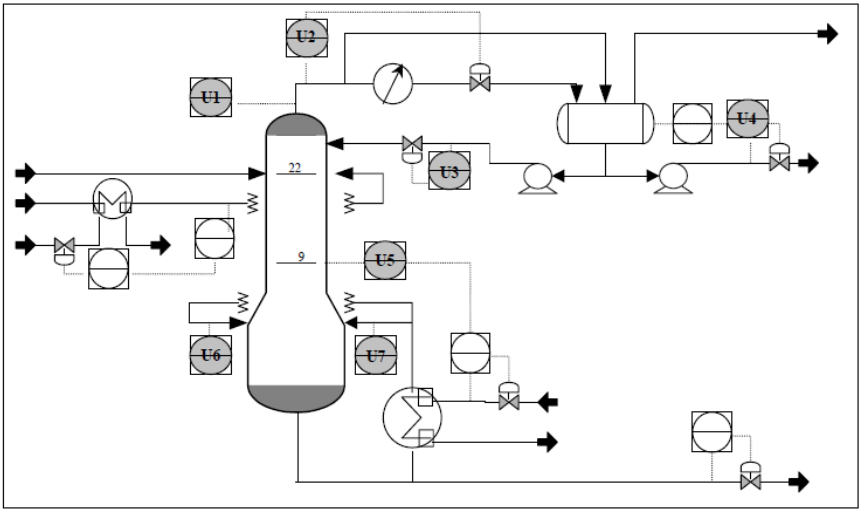
\includegraphics[width=0.5\textwidth]{images/TTT.png}
  \caption{脱丁烷塔示意图} 
\end{figure}

在这个过程中安装了一些传感器对过程变量进行测量,以监控产品质量。测量的变量在下表1中列出。这些变量也就是上图2中的灰色变量 U1-U7。测量变量描述如下:

\begin{itemize}
  \item U1:Top temperature
  \item U2:Top pressure
  \item U3:Reflux flow
  \item U4:Flow to next process
  \item U6:Bottom temperature
  \item U7:Bottom temperature
\end{itemize}

脱丁烷塔底部的丁烷含量,也就是我们需要监控(预测)的变量,因为这关系到产品的质量。丁烷含量的真实值是
在脱异戊二烯塔的上方测量得到的,也就是图1中 Plant C 的 $A2$ 部分测量得到的($C4$ in $C5(\%)$)。我们需要建立
软测量模型,通过 $U1\sim U7$ 的测量变量的值,对塔底丁烷含量(质量变量)进行预测。这个过程具有较强的动态性,可以
理解为 $t$ 时刻样本与其之前 $t-1,t-2,\dots$ 的样本有很强的关联,如果能挖掘出变量间的动态信息,对预测精度的提升会有很大帮助。

\subsection{数据集介绍}

\begin{enumerate}
  \item 本数据集中包含4个文件,其中 \lstinline{train_input} 为训练集的输入(特征/测量变量);\lstinline{train_output} 为
  训练集的输出(质量变量);\lstinline{test_input} 为测试集输入(特征/测量变量);数据上
  交模板为提交模板,用户需利用训练集建立模型,完成所有测试样本的预测并将结果按照模板格式进行保存并在系统中提交。
  \item 训练集中样本个数为1596(7个特征,1个标签),测试样本个数为 798(7个特征,无标签)。数据训
  练集和测试集在时间上是连续的(测试表1测量变量描述样本在时间上是接着训练样本进行采样的),由于工业现
  场数据采集过程存在中断,干扰等原因,训练集和测试样本有一定比例的缺失值,数据集中已经用“nan”进行标
  识,缺失比例大概在 3\%左右,用户需尽可能地利用缺失数据的信息。
  \item 数据每个特征代表的含义已在上表中列出,训练集最后一列为标签:丁烷含量。
  \item 评价指标采用均方根误差(\lstinline{RMSE}),误差越低,排名越高。
\end{enumerate}

\section{数据分析}

在刚刚接触到项目时,我们最为注重数据分析与数据预处理方面的操作。根据目前已有的一些经验,
一个合理的数据分析往往可以起到事半功倍的效果,它不仅可以为数据预处理指明方向,极大地提高
数据质量,更有助于模型取得优秀的预测成绩。

针对关键变量脱丁烷塔底部的丁烷含量所选择的七个辅助变置分别为:塔顶温度、塔顶压力、回流流量、下级流量、第六层的温度、塔底两侧温度。测量变量包含两个流量、一个压力、四个温度。

我们的想法是,先通过不同维度数据的相关程度以及分布进行分析,再从中寻找能够有效表示特征的维度,
进而在后序的数据预处理与模型搭建中着重考虑。

\begin{figure}[H]
  \centering
  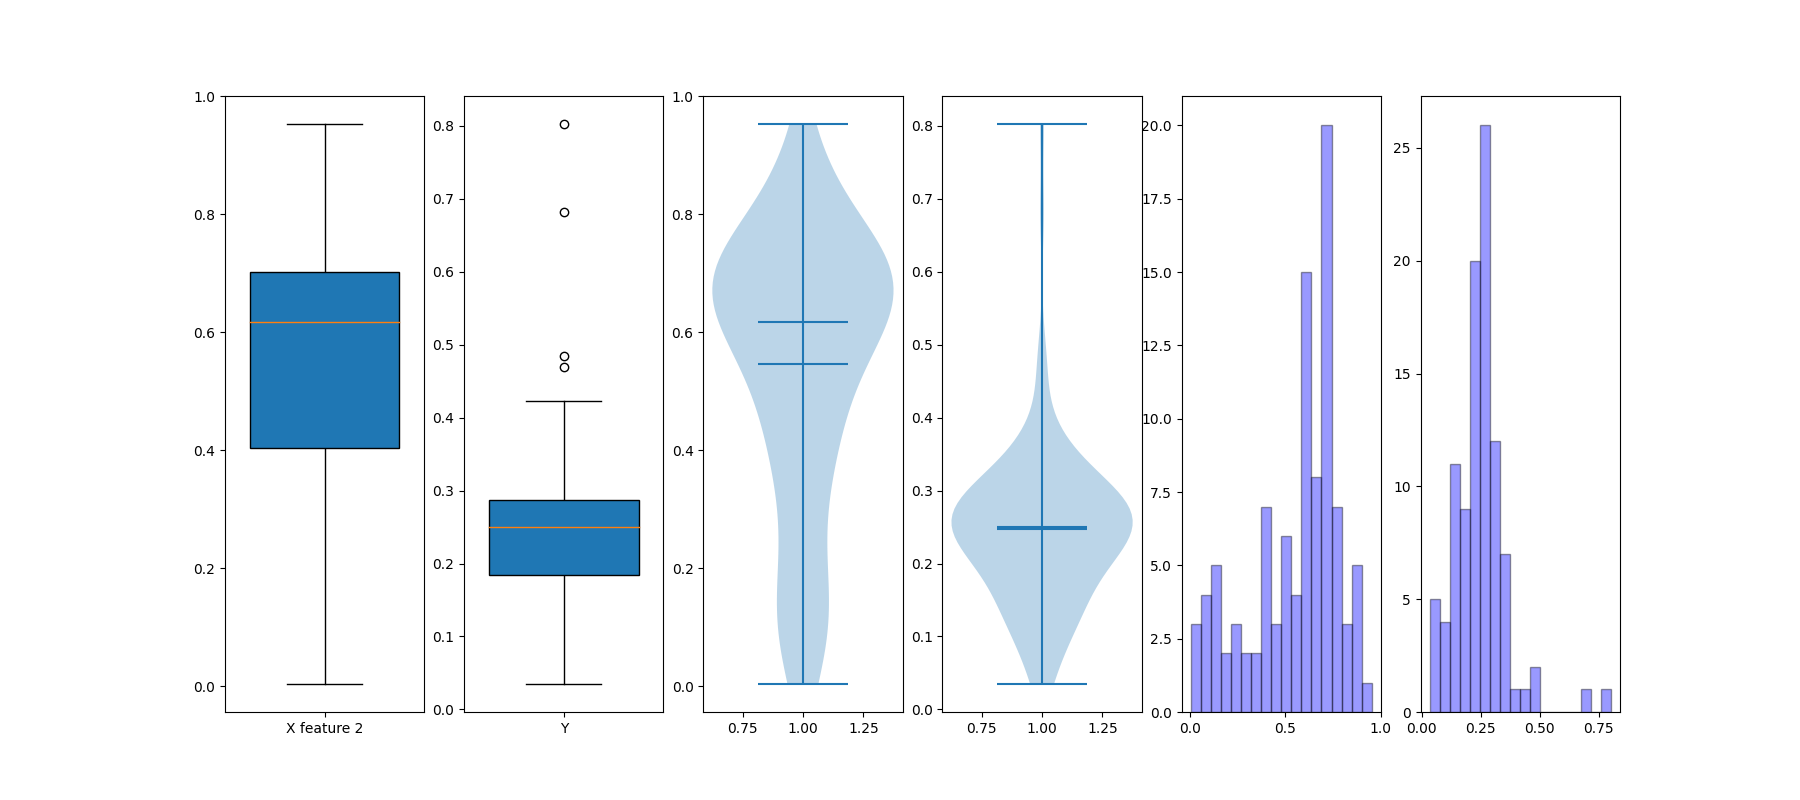
\includegraphics[width=0.5\textwidth]{images/single_feature.png}
  \caption{单个维度数据与最终输出的关系-1} 
\end{figure}

\begin{figure}[H]
  \centering
  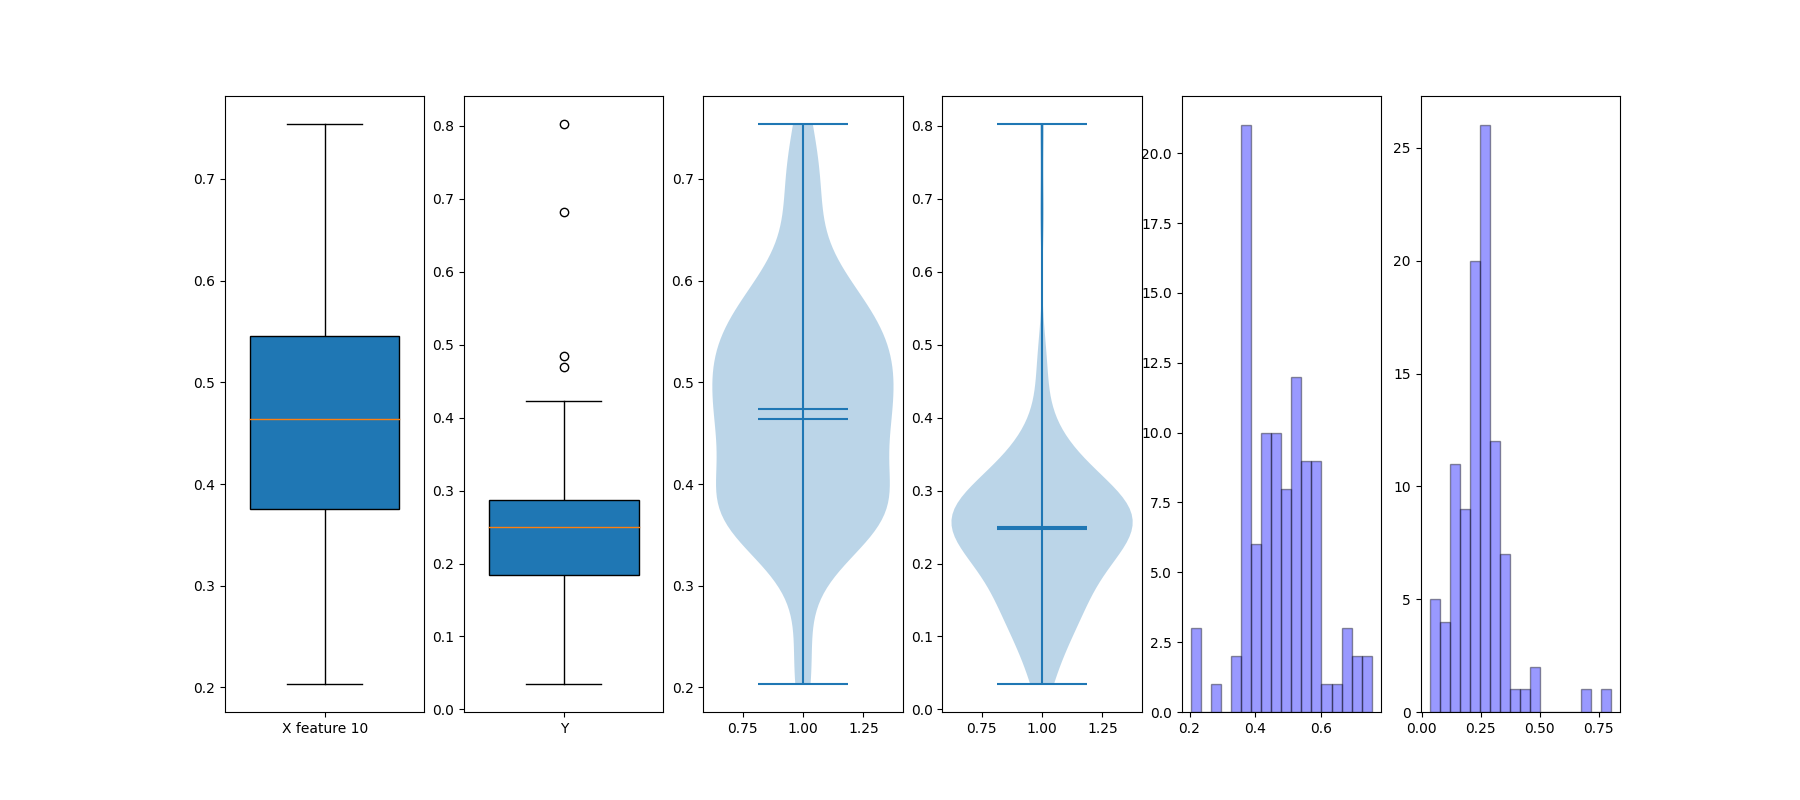
\includegraphics[width=0.5\textwidth]{images/single_feature_1.png}
  \caption{单个维度数据与最终输出的关系-2} 
\end{figure}

上方两张图是关于单个维度数据与最终输出的数据分布的对比图,通过对7个维度的分析,我组认为
第3、5、7维度的数据具有较明显的特征。但是这仅仅是空间上的特征,对于一个时序数据,仅仅提取空间上的
特征是远远不够的,所以我们想到分析此时刻与之前两个时刻的一共21个特征的相关关系。

\begin{figure}[H]
  \centering
  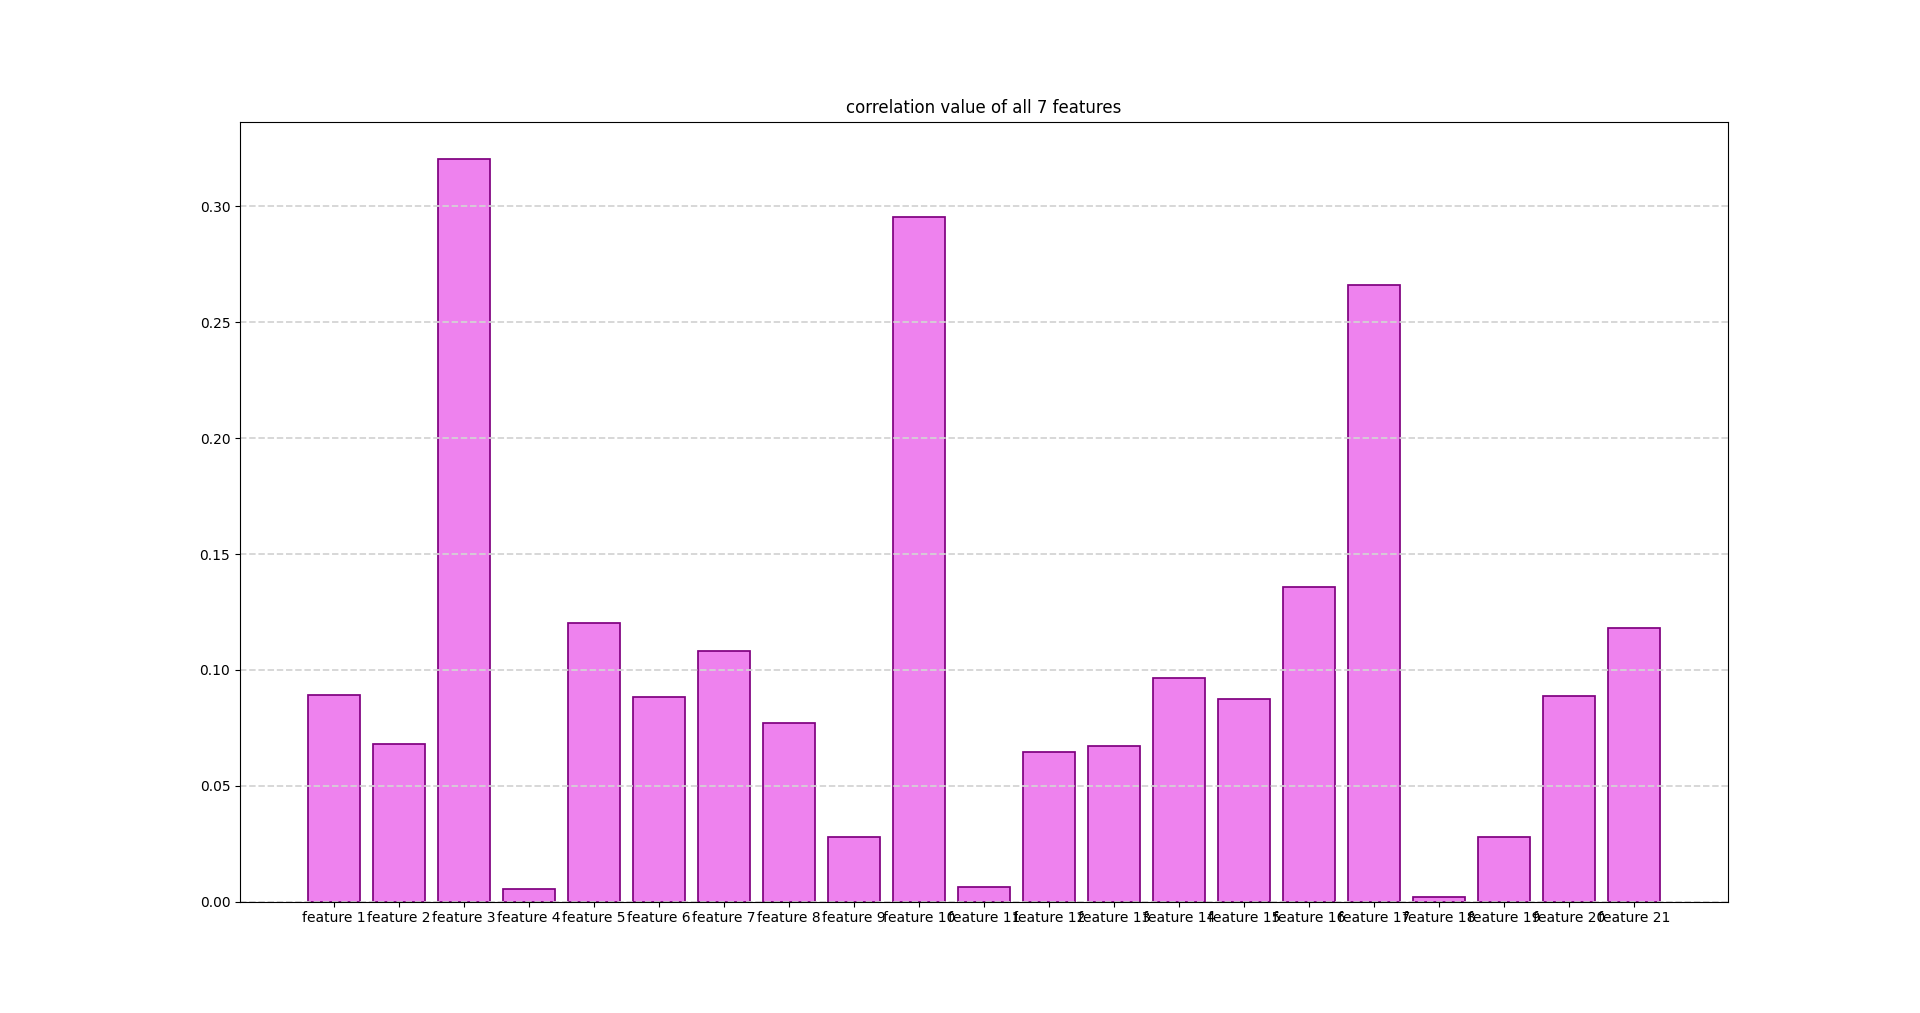
\includegraphics[width=0.5\textwidth]{images/CORR.png}
  \caption{三个时刻21个维度与输出的相关关系} 
\end{figure}

\begin{figure}[H]
  \centering
  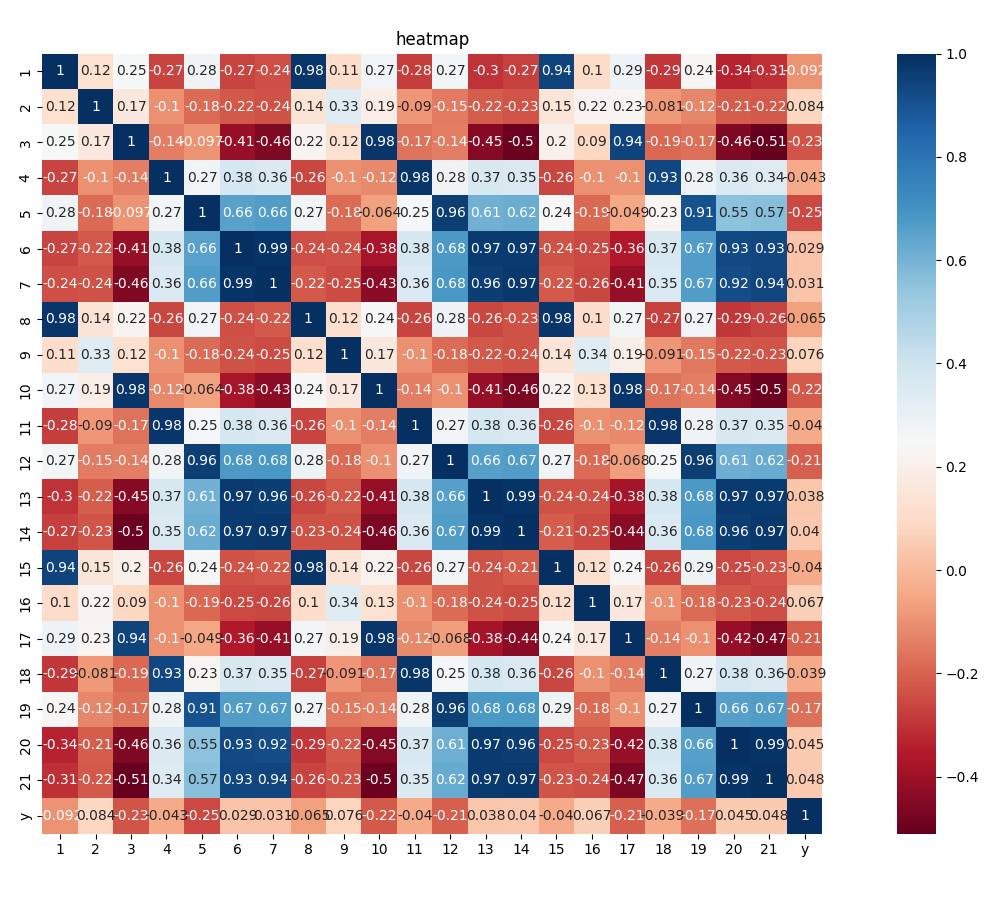
\includegraphics[width=0.5\textwidth]{images/HEAT.png}
  \caption{三个时刻21个维度与输出的热力图} 
\end{figure}

从图中我们发现了一个有意思的现象:假设当前时刻为$t$,$t-2$时刻的维度3与最终结果的相关关系高于$t-1$时刻与$t$时刻的维度3;
$t-2$时刻的维度5与最终结果的相关关系同样高于$t-1$时刻与$t$时刻的维度5;但是对于维度2,$t$时刻与输出最为相关,其次是
$t-2$时刻,$t-1$时刻。这些信息表明,前几个时刻的数据往往比当前时刻具有更有效的特征。我们还分析了再往前20个时刻的特征,
但是综合权衡预测准确度以及计算机算力后,我们最终使用三个时刻的数据进行综合处理,生成一个数据后再放入\lstinline{LSTM}
、\lstinline{CNN}等模型中
进行脱丁烷塔的温度预测。

\section{数据预处理}

\subsection{特征合并}

对于这个七维的数据空间,我们希望可以找到一个$M$($M < 7$)维的正交向量,让七维空间映射过去后,还可以尽量多的保持原有数据空间的信息量。此时首选运用主成分分析对数据进行处理,代码如下:

\begin{lstlisting}[language=Python]
def pca_data(data):
    from sklearn.decomposition import PCA
    pca = PCA()
    pca.fit(data)
    PCA(copy=True, n_components=None, whiten=False)
    # 返回模型的各个特征向量
    print(pca.components_)  
    print("*" * 50)
    # 返回各个成分个字的方差百分比
    print(pca.explained_variance_ratio_)  
    return pca.explained_variance_ratio_
\end{lstlisting}

\lstinline{pca.explained_variance_ratio_}计算了每个特征方差贡献率,所有总和为1。
这个比例越大,则越是重要的主成分。通过结果\lstinline{[0.5723516 0.23383997 0.09696936 0.06866214 0.01678858 0.00948701 0.00190138]},
我们可以看出最后几个特征方差贡献率较低。考虑合并不重要的特征,减少特征间的相关系数。

在做了相关性分析后,我们发现第六和第七个特征相关系数很高,查看实际意义后发现这两个特征分别代表塔底部左右两边的温度,所以选择对第六个和第七个求取平均值变为一个特征。该特征可以近似为塔底中心温度。避免了变量间相关系数过高的问题。


\subsection{去除异常值}

异常值,即在数据集中存在不合理的值,又称离群点。常见判别方法有:

\begin{enumerate}
  \item 简单统计分析:对属性值进行一个描述性的统计,从而查看哪些值是不合理的。
  \item $3\sigma$原则:当数据服从正态分布时,
  根据正态分布的定义可知,距离平均值$3\sigma$之外的概率为 $P(|x-\mu|>3\sigma) \leqslant 0.003$,这属于极小概率事件,在默认情况下我们可以认定
  距离超过平均值$3\sigma$的样本是不存在的。 因此,当样本距离平均值大于$3\sigma$,则认定该样本为异常值。
  当数据不服从正态分布,可以通过远离平均距离多少倍的标准差来判定,多少倍的取值需要根据经验和实际情况来决定。
  \item 箱型图分析:箱型图提供了一个识别异常值的标准,即大于或小于箱型图设定的上下界的数值即为异常值。箱型图选取异常值比较客观,在识别异常值方面有一定的优越性。
\end{enumerate}

由于异常值带微弱主观性,判定没有固定标准,一些异常值也可能同时包含有用的信息,是否需要剔除,应由分析人员自行判断。为了保留更多信息防止错误去除,我们只是简单地将超出$(0,1)$范围内的数据点认为是缺失值。

异常值的处理方法常用有四种:

\begin{enumerate}
  \item 删除含有异常值的记录
  \item 将异常值视为缺失值,交给缺失值处理方法来处理
  \item 用平均值来修正
  \item 不处理
\end{enumerate}

但是总数据样本较少而且样本在时间上连续,直接剔除显然是不合理的做法。包含异常值的样本也应该得到充分利用,我们选择第二种方法进行处理,将异常值修改为缺失值。


\subsection{弥补缺失值}

使用\lstinline{SPSS}对所给数据进行分析,训练集的缺失值统计如下:

\begin{figure}[H]
  \centering
  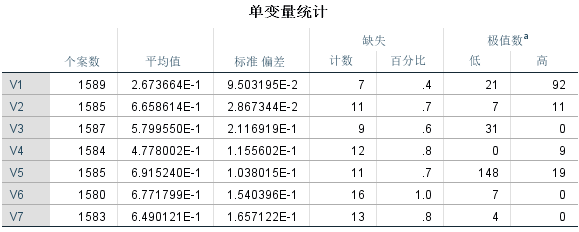
\includegraphics[width=0.5\textwidth]{images/QQQ.png}
  \caption{训练集缺失值的单变量统计}
\end{figure}

我们组一共采用了三种方法对缺失值进行填补:

\subsubsection{简单补零}

下图为缺失值补零后七个特征的时序图,可见这种方法使得填补后特征不够连续,可能会影响后续模型训练,应选择其他方法重新填补。

\begin{figure}[H]
  \centering
  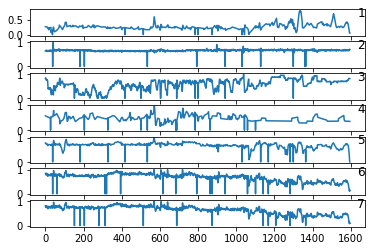
\includegraphics[width=0.5\textwidth]{images/ZERO.png}
  \caption{补零后的7特征时序图}
\end{figure}

\subsubsection{拉格朗日插值}

已知函数$y=f(x)$在$n+1$个不同的点$x_0 ,x_1 ,\dots ,x_n$上的函数值分别为$y_0, y_1, \dots,y_n$,一个次数
不超过$n$的多项式$P_n(x)$,使其满足: $P_n(x_i)=y_i\quad (i=0,1,\dots,n)$。
即$n+1$个不同的点可以唯一决定一个$n$次多项式。

\begin{lstlisting}[language=Python]
def ployinterp_column(s,i,n):
    # 自定义列向量插值函数
    from scipy.interpolate import lagrange
    k = 3
    #print(s.shape)
    # 取前后k个数的索引
    a=s[i][np.arange(n-k,n)]
    b=s[i][np.arange(n+1,n+1+k)]
    #2k个点
    y=np.hstack((a,b))
    #y = y[y.notnull()] # 剔除空值
    #2k个点对应坐标
    x=np.hstack((np.arange(n-k,n),np.arange(n+1,n+1+k)))
    # 返回这2k个数据的拉格朗日多项式函数在n的值
    return lagrange(x,y)(n)
\end{lstlisting}

得到的统计结果图如下,拉格朗日插值结果相较于直接补零有极大改善,但该方法插值仍然容易预测出离谱结果,图像上存在一些尖峰,需要特殊处理。

\begin{figure}[H]
  \centering
  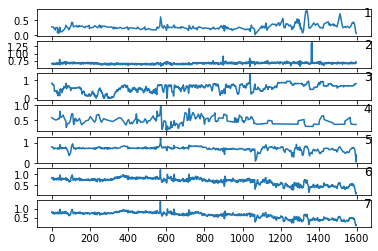
\includegraphics[width=0.5\textwidth]{images/LLL.png}
  \caption{拉格朗日插值后的7特征时序图}
\end{figure}


\subsubsection{随机森林}

对于一个有$n$个特征的数据来说,其中特征$T$有缺失值,我们就把特征$T$当作标签,
其他的$n-1$个特征和原本的标签组成新的特征矩阵。
对于$T$来说,它没有缺失的部分,就是我们的$y\_test$,这部分数据既有标签也有特征,而它缺失的部分,
只有特征没有标签,就是我们需要预测的部分。

然而给定数据中有多个特征有缺失值,我们的选择是遍历所有的特征,从缺失最少的开始进行填补(因为
填补缺失最少的特征所需要的准确信息最少)。填补一个特征时,先将其他特征的缺失值用0代替,每完成一次回归预测,
就将预测值放到原本的特征矩阵中,再继续填补下一个特征。每一次填补完毕,有缺失值的特征会减少一个,所以每次循环后
,需要用0来填补的特征就越来越少。当进行到最后一个特征时(这个特征应该是所有特征中缺失值最多的),已经没有任何的
其他特征需要用0来进行填补了,而我们已经使用回归为其他特征填补了大量有效信息,可以用来填补缺失最多的特征。

为了利用好训练集中对应预测数据(脱丁烷塔含量)的信息,将其也加入预测其他变量缺失值的特征,代码如下:

\begin{lstlisting}[language=Python]
def RandomForest(a,b):
  import numpy as np
  import pandas as pd
  import matplotlib.pyplot as plt
  from sklearn.impute import SimpleImputer#填补缺失的类
  from sklearn.ensemble import RandomForestRegressor
  x_full = a     #x.shape = (1596, 7)
  y_full = b
  n_samples = 1596    #样本数量
  n_features = 7  #标签数量
  x_full = pd.DataFrame(x_full)
  x_missing_reg = x_full.copy() #随机森林的填补的结果放在x_missing_reg
  #使用np.argsort将缺失值从少到多进行排序
  sortindex = np.argsort(x_missing_reg.isnull().sum(axis=0)).values
  print (sortindex)
  for i in sortindex:
      #构建新特征矩阵(没有被选中去填充的特征+原始的标签)和新标签(被选中去填充的特征)
      df = x_missing_reg
      fillc = df.iloc[: , i]
      df = pd.concat([df.iloc[: , df.columns != i] , pd.DataFrame(y_full)] , axis=1)

      #在新特征矩阵中,对含有缺失值的列,进行0的填补
      df_0 = SimpleImputer(missing_values=np.nan , strategy="constant" , fill_value=0).fit_transform(df)
      
      #构建新的训练集和测试集
      y_train = fillc[fillc.notnull()]#被选中要填充的值,非空值
      y_test = fillc[fillc.isnull()]#是被选中的要填充给的值,是空值
      x_train = df_0[y_train.index,:]#非空值所对应的的索引
      x_test = df_0[y_test.index,:]#空值所对应的记录
      #用随机森林填补缺失值
      rfc = RandomForestRegressor(n_estimators=100)#实例化
      rfc = rfc.fit(x_train,y_train)  #导入训练集去进行训练
      y_predict = rfc.predict(x_test) #用predict接口将x_test导入,得到我们的预测结果,此结果就是要用来填补空值的
      #print(y_predict)
      #将填补好的特征返回到我们的原始的特征矩阵中
      x_missing_reg.loc[x_missing_reg.iloc[:,i].isnull() , i] = y_predict
      #print (x_missing_reg)
  return x_missing_reg
\end{lstlisting}

针对测试集的缺失值,由于没有真实结果,所以仅考虑利用七个特征间的关系来进行随机森林插值,由于原理相似,此处不再展示相关函数。


\subsubsection{转换为监督学习问题}

针对数据具有时序性和时滞性的特点,预测时需要历史信息。

解决方法是时序拓展。预测当前时刻的目标值时用到前$n$个时刻的特征数据:

\begin{enumerate}
  \item 设定时间窗口长度
  \item 按照时间窗口长度合并特征
  \item 得到时间窗划分后的特征变量
\end{enumerate}

下面的函数的作用是加入前$n\_in$个时间点的特征值,预测$n\_out$时间后的特征。

\begin{lstlisting}[language=Python]
def series_to_supervised(data, n_in, n_out):
  """
  数据处理
  :param data:数据
  :param n_in:输入特征个数
  :param n_out:目标值
  :param dropnan:是否删除 Nan 值 
  :return:
  """
  df = pd.DataFrame(data)
  n_vars = df.shape[1]  # n_vars 列数
  cols, names = list(), list()
  
  # 时间间隔跨度, 时间点个数,共 n_in 个
  # 首先添加当前时刻之前的时间点
  for i in range(n_in - 1, 0, -1):
      cols.append(df.shift(i))
      names += [('var%d(t-%d)' % (j + 1, i)) for j in range(n_vars)]
  # 然后添加当前时刻
  cols.append(df)
  names += [('var%d(t)' % (j + 1)) for j in range(n_vars)]

  # 添加 target 为未来 n_out 分钟后时刻的温度
  cols.append(df.shift(-n_out))
  names += [('var%d(t+%d)' % (j + 1, n_out)) for j in range(n_vars)]
  agg = pd.concat(cols, axis=1)
  agg.columns = names
  # 删除缺失值
  agg.dropna(inplace=True)

  return agg
\end{lstlisting}

得到的统计结果图如下,随机森林插值结果相较于前两种方法曲线更为平滑,我们最终选用这种方法。

\begin{figure}[H]
  \centering
  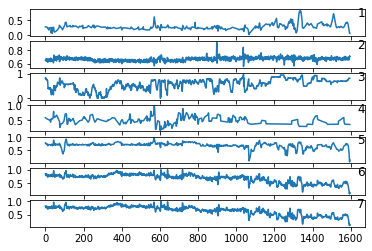
\includegraphics[width=0.5\textwidth]{images/FFF.png}
  \caption{时序拓展后的7特征时序图}
\end{figure}

\section{模型搭建}

\subsection{最小二回归(OLS)}

\lstinline{OLS}全称\lstinline{ordinary least squares},
是回归分析(\lstinline{regression analysis})最根本的一个形式,对模型条件要求最少,
也就是使散点图上的所有观测值到回归直线距离的平方和最小。

在《传感与检测》课程中,我们学习到:软测量模型的一个基本方法就是进行回归分析。
而最小二乘回归又是回归分析中最基础最实用的一种基本方法,因此我们有必要先使用最小二乘回归来初步解决问题。
在正式实现之前,我们先对其进行初步的理论分析。

这里,我们将会给出\lstinline{OLS}在矩阵形式下的一般通解。

当样本数据有$n$个时,有如下的线性方程组:

$$
\left\{\begin{array}{l}
a x_{1}+b=y_{1} \\
a x_{2}+b=y_{2} \\
a x_{3}+b=y_{3} \\
\cdots \\
a x_{n}+b=y_{n}
\end{array}\right.
$$

简单改写成矩阵形式即为:

$$
\left[\begin{array}{cc}
x_{1} & 1 \\
x_{2} & 1 \\
x_{3} & 1 \\
\vdots & \vdots \\
x_{n} & 1
\end{array}\right]\left[\begin{array}{l}
a \\
b
\end{array}\right]=\left[\begin{array}{c}
y_{1} \\
y_{2} \\
y_{3} \\
\vdots \\
y_{n}
\end{array}\right]
$$

令:

$$
X=\left[\begin{array}{cc}
x_{1} & 1 \\
x_{2} & 1 \\
x_{3} & 1 \\
\vdots & \vdots \\
x_{n} & 1
\end{array}\right], \beta=\left[\begin{array}{c}
a \\
b
\end{array}\right], Y=\left[\begin{array}{c}
y_{1} \\
y_{2} \\
y_{3} \\
\vdots \\
y_{n}
\end{array}\right]
$$

则得到:

$$
X\cdot \beta = Y
$$

在矩阵形式中,我们的目标是找到一个向量$\beta$,使得$X\cdot\beta-Y$的欧几里得范数最小,那么:

$$
\begin{aligned}
S &=\|X \cdot \beta-Y\|_{2}^{2} \\
&=[X \cdot \beta-Y]^{\mathrm{T}} \cdot[X \cdot \beta-Y] \\
&=\left[(X \cdot \beta)^{\mathrm{T}}-Y^{\mathrm{T}}\right] \cdot[X \cdot \beta-Y] \\
&=\left[\beta^{\mathrm{T}} \cdot X^{\mathrm{T}}-Y^{\mathrm{T}}\right] \cdot[X \cdot \beta-Y] \\
&=\beta^{\mathrm{T}} \cdot X^{\mathrm{T}} \cdot X \cdot \beta-\beta^{\mathrm{T}} \cdot X^{\mathrm{T}} \cdot Y-Y^{\mathrm{T}} \cdot X \cdot \beta+Y^{\mathrm{T}} \cdot Y
\end{aligned}
$$

推导得到:

$$
S=\beta^{\mathrm{T}} \cdot X^{\mathrm{T}} \cdot X \cdot \beta-2 \cdot Y^{\mathrm{T}} \cdot X \cdot \beta+Y^{\mathrm{T}} \cdot Y
$$

同样地,我们对$\beta$求偏导:

$$
\begin{aligned}
\frac{\partial S}{\partial \beta} &=\frac{\partial\left(\beta^{\mathrm{T}} \cdot X^{\mathrm{T}} \cdot X \cdot \beta-2 \cdot Y^{\mathrm{T}} \cdot X \cdot \beta+Y^{\mathrm{T}} \cdot Y\right)}{\partial \beta} \\
&=\frac{\partial\left(\beta^{\mathrm{T}} \cdot X^{\mathrm{T}} \cdot X \cdot \beta\right)}{\partial \beta}-2 \cdot \frac{\partial\left(Y^{\mathrm{T}} \cdot X \cdot \beta\right)}{\partial \beta}+\frac{\partial\left(Y^{\mathrm{T}} \cdot Y\right)}{\partial \beta}
\end{aligned}
$$

利用矩阵求导的相关公式:

$$
\left\{\begin{array}{l}
\frac{\partial\left(x^{\mathrm{T}} \cdot a\right)}{\partial x}=\frac{\partial\left(a^{\mathrm{T}} \cdot x\right)}{\partial x}=a \\
\frac{\partial\left(x^{\mathrm{T}} \cdot B \cdot x\right)}{\partial x}=\left(B+B^{\mathrm{T}}\right) \cdot x
\end{array}\right.
$$

上式可简化为:

$$
\begin{aligned}
\frac{\partial S}{\partial \beta} &=\left[X^{\mathrm{T}} \cdot X+\left(X^{\mathrm{T}} \cdot X\right)^{\mathrm{T}}\right] \cdot \beta-2 \cdot\left(Y^{\mathrm{T}} \cdot X\right)^{\mathrm{T}} \\
&=\left[X^{\mathrm{T}} \cdot X+X^{\mathrm{T}} \cdot X\right] \cdot \beta-2 \cdot X^{\mathrm{T}} \cdot Y \\
&=2 \cdot X^{\mathrm{T}} \cdot X \cdot \beta-2 \cdot X^{\mathrm{T}} \cdot Y
\end{aligned}
$$

令其为0,如果$(X^T\cdot X)^{-1}$存在,则参数$\beta$在\lstinline{OLS}下的通解如下:

$$
\begin{aligned}
&X^{\mathrm{T}} \cdot X \cdot \beta-X^{\mathrm{T}} \cdot Y=0 \\
&\Rightarrow X^{\mathrm{T}} \cdot X \cdot \beta=X^{\mathrm{T}} \cdot Y \\
&\Rightarrow\left(X^{\mathrm{T}} \cdot X\right)^{-1} \cdot\left(X^{\mathrm{T}} \cdot X\right) \cdot \beta=\left(X^{\mathrm{T}} \cdot X\right)^{-1} \cdot X^{\mathrm{T}} \cdot Y \\
&\Rightarrow \beta=\left(X^{\mathrm{T}} \cdot X\right)^{-1} \cdot X^{\mathrm{T}} \cdot Y
\end{aligned}
$$

方便的是,在\lstinline{Python}的常用库中,我们可以使用\lstinline{statsmodels}库函数来简单完成上述的拟合过程。
在去除数据集中的异常数值后,我们完成了对模型的基本拟合。使用\lstinline{model.summary}方法可以简便地观察数据集和我们的拟合结果。

\begin{lstlisting}[language=Python]
import statsmodels.api as sm
x=sm.add_constant(x)
est=sm.OLS(y,x)
# 建立最小二乘回归模型
model=est.fit() 
print(model.summary())
y_fitted = model.fittedvalues
fig, ax = plt.subplots(figsize=(8,6))
ax.plot(y, '--', label='data')
ax.plot(y_fitted, '-',label='OLS')
ax.legend(loc='best')
\end{lstlisting}

\begin{figure}[H]
  \centering
  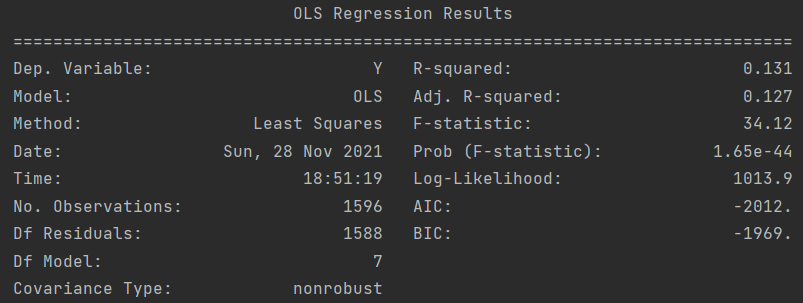
\includegraphics[width=0.5\textwidth]{images/OLS.png}
  \caption{\lstinline{OLS}处理结果} 
\end{figure}

在训练集上简单拟合如图所示,观察到\lstinline{OLS}并不能很好拟合所有的点。
因为\lstinline{OLS}的拟合结果衡量标准是欧几里得范数,这还是一个相对简单的模型。因此其拟
合结果不会准确地落在一些较高和较低的位置,整体模型参数也较少。

\begin{figure}[H]
  \centering
  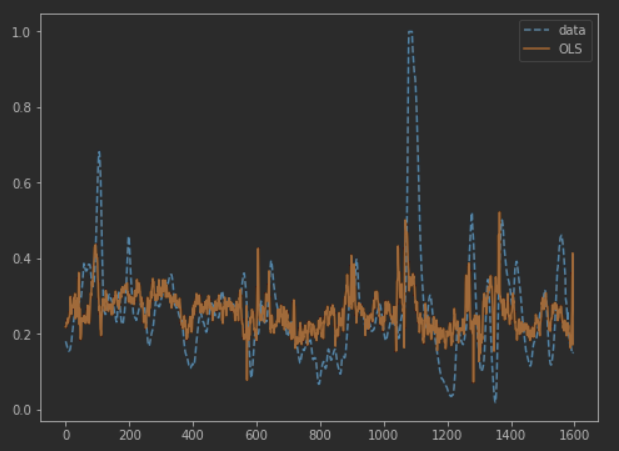
\includegraphics[width=0.5\textwidth]{images/F.png}
  \caption{\lstinline{OLS}模型对验证集的拟合} 
\end{figure}

用\lstinline{OLS}模型对测试集进行拟合,不出意外,拟合结果分布较为杂乱,
测试分数\lstinline{RMSE}分数也不尽人意。其本质原因还是\lstinline{OLS}的参数太少以及其优化
目标——欧几里得范数最小并不能适应我们的数据样本。其中的非线性因素比如噪声、冗余
变量以及时序关系是该模型所不能处理的。因此我们要在后面的模型尝试中逐渐解决这些问题。

值得一提的是,\lstinline{statsmodels}库实现了模型的简单调用和拟合,这是其他方法所不能具备的巨大优势,节约了我们很多编程时间。

\lstinline{statsmodels}是一个 \lstinline{Python} 模块,它提供用于估计许多不同统计模型以及进行统计测试和统计数据探索的类和函数。
\lstinline{statsmodels}支持使用 \lstinline{R} 样式公式和\lstinline{pandasDataFrame}指定模型。

\begin{lstlisting}[language=Python]
from matplotlib import pyplot as plt
import statsmodels.api as sm
y_test = model.predict(xx)
fig, ax = plt.subplots(figsize=(8,6))
ax.plot(y_test, '-',label='OLSPreD')
ax.legend(loc='best')
\end{lstlisting}

\begin{figure}[H]
  \centering
  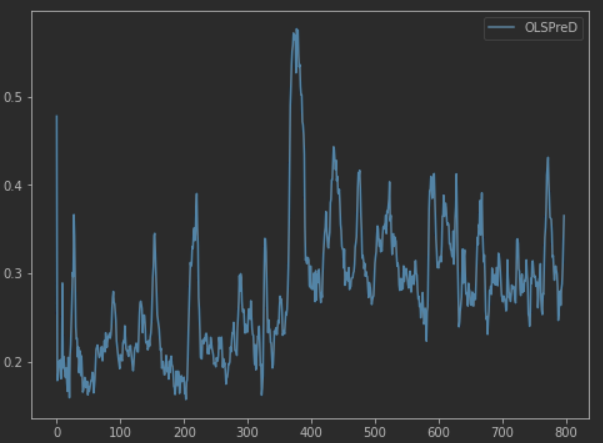
\includegraphics[width=0.5\textwidth]{images/FF.png}
  \caption{\lstinline{OLS}模型对测试集的拟合} 
\end{figure}

\subsection{偏最小二乘回归(PLS)}

前文提到,在进行本问题的回归分析时,尤其是当我们的样本数据特征存在多重共线性问题时,
普通的多元线性回归无法很好的解决问题。因此我们有必要使用偏最小二乘法回归,它能帮助我们实现减小样本之间相关关系的目标。

\lstinline{PLS}回归(\lstinline{Partial least squares regression},偏最小二乘法回归)是一种解决共线性问题、
多个因变量\lstinline{Y}同时分析、以及处理小样本时影响关系研究的一种多元统计方法。

\lstinline{PLS}回归集合了主成分分析、典型相关、多元线性回归三者于一。简单说明,\lstinline{PLS}的原理可以理解为:

\lstinline{PLS}回归运用主成分分析的原理,将多个$X$和多个$Y$,分别浓缩为成分($X$对应主成分$U$,$Y$对应主成分$V$),然后借助于典
型相关原理,可分析$X$与$U$的关系,$Y$与$V$的关系;以及结合多元线性回归原理,分析$X$对于$V$的关系,从而研究到$X$对于$Y$的关系。

在进行回归分析时,理论上要求因变量正态,并且样本量不能太小等。我们希望研究相关变量之间的影响关系,此时则可以使用\lstinline{PLS}回归。

\lstinline{PLS}的准则函数通俗的讲就是提取主元时所按照的准则,与PCA不同,\lstinline{PLS}在提取主元时考虑的不仅是
能最大程度概括自变量空间的数据信息,还应该考虑自变量主元对于因变量变化的解释作用。

偏最小二乘的一般多元底层模型是:

$$
\begin{aligned}
&X=T P^{\top}+E \\
&Y=U Q^{\top}+F
\end{aligned}
$$

其中X是一个$n*m$的预测矩阵,$Y$是一个$n*p$的响应矩阵。
$T$和$U$是$n*l$的矩阵,分别为$X$的投影(“X分数”、“组件”或“因子”矩阵)和$Y$的投
影(“$Y$分数”)。$P$和$Q$分别是$m*l$和$p*l$的正交载荷矩阵,以及矩阵$E$和$F$是误差项,服从
独立同分布的正态分布随机变量。对X和Y分解来最大化$T$和$U$之间的协方差。

对于我们来说,\lstinline{PLS}的步骤简单来讲,有如下过程:

\begin{enumerate}
  \item 数据说明与标准化
  \item 求符合要求的主成分(这一步是关键)
  \item 建立主成分与原自变量、因变量之间的回归(这一步也是关键)
  \item 继续求主成分,直到满足要求
  \item 推导因变量之于自变量的回归表达式(这一步也很重要)
  \item 交叉有效性检验
\end{enumerate}

本案例研究中,脱丁烷塔各个位置的测量值同属一个生产过程,因此其有很强的相关性。
而且我们的样本数量只有1500个左右,不算太大也不算太小,因此可以使用\lstinline{PLS}来进行研究。

\begin{figure}[H]
  \centering
  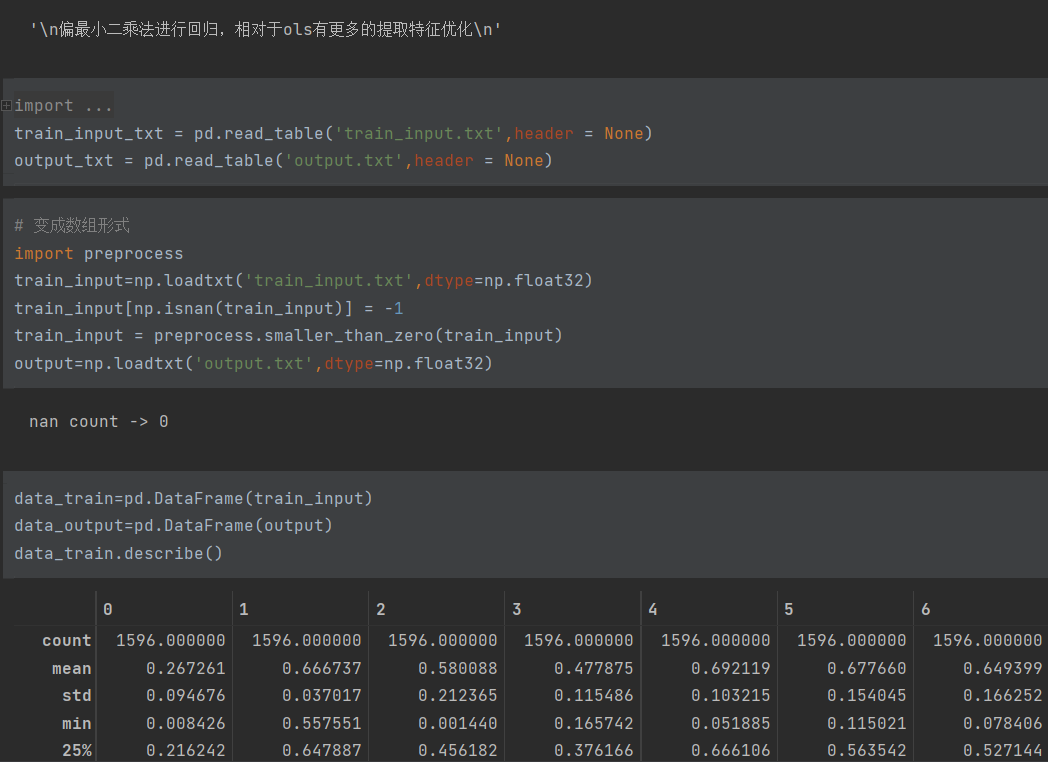
\includegraphics[width=0.5\textwidth]{images/P.png}
  \caption{\lstinline{PLS}数据预处理} 
\end{figure}

首先这里还是进行最基本的数据预处理,要消除异常值对模型的影响。
其次,上文提到,\lstinline{statsmodels.api}给我们提供了很利于研究处理的框架,我们可以使用其中的方法来简单完成。


\begin{lstlisting}[language=Python]
from matplotlib import pyplot as plt
from sklearn.cross_decomposition import PLSRegression
from sklearn.model_selection import GridSearchCV
import statsmodels.api as sm
# pls = PLSRegression(n_components=3, max_iter=500)
pls = PLSRegression()
param_grid = {
    "n_components": [3, 4, 5, 6, 7],
    "tol": [0.001, 0.0001, 0.00001, 0.000001, 0.0000001],
    "max_iter": [500, 600, 700, 800, 900, 1000]
}
x = data_train[['A','B','C','D','E','F','G']]
y = data_output[['Y']]
clf = GridSearchCV(pls, param_grid=param_grid)
clf.fit(x, y)
print("best estimator ->", clf.best_estimator_)
\end{lstlisting}

其中,\lstinline{from sklearn.cross_decomposition import PLSRegression}这一句则用到了我们
的老朋友\lstinline{sklearn}库。\lstinline{sklearn}是一个\lstinline{Python}第三方提供的非常强力的机器学习库,它包含
了从数据预处理到训练模型的各个方面。在实战使用\lstinline{scikit-learn}中可以极大的节省我们编
写代码的时间以及减少我们的代码量,使我们有更多的精力去分析数据分布,调整模型和修改
超参。但是实际上,我这里的这两句:

\begin{lstlisting}[language=Python]
# pls = PLSRegression(n_components=3, max_iter=500)
pls = PLSRegression()
\end{lstlisting}

并没有使用其函数的参数设置,而是让它自己去选择特征元数量,然后自行拟合,这也是\lstinline{sklearn}库一个十分便捷的地方。
这里,\lstinline{PLSRegression}方法也自行计算出了我们需要的结果,展示在下方。

\begin{figure}[H]
  \centering
  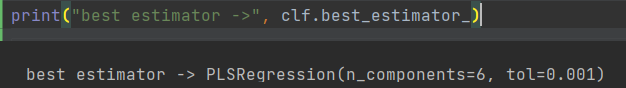
\includegraphics[width=0.5\textwidth]{images/PP.png}
  \caption{\lstinline{PLS}自动估算最优参数} 
\end{figure}

这里,对\lstinline{PLS}的拟合模型效果进行展示,从宏观上能发现,\lstinline{PLS}对数据整体的特征抓取能力更强,
对某些较高和较低点,相对于\lstinline{OLS}也有了较
大幅度的变动,这令人心中一喜。后面发现其\lstinline{RMSE}值也比\lstinline{OLS}的值有了略微的降低,
这正是模型减少了冗余特征的影响。

\begin{figure}[H]
  \centering
  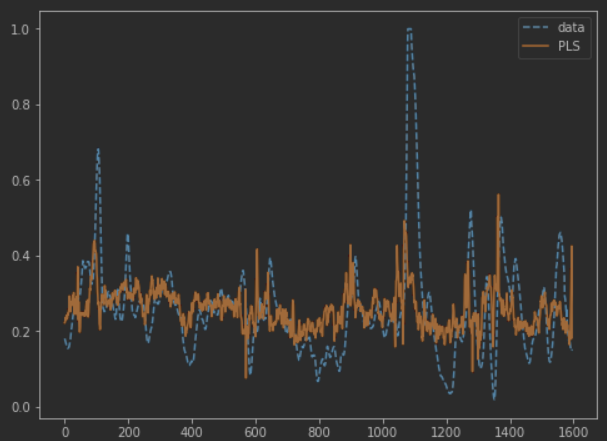
\includegraphics[width=0.5\textwidth]{images/PPP.png}
  \caption{\lstinline{PLS}模型对验证集的拟合} 
\end{figure}

接下来,对保存的\lstinline{model}用\lstinline{predict}方法就可以简单对测试集进行预测了。从宏观上看来,
数据预测结果依旧还是比较杂乱的,但是其\lstinline{RMSE}的值略微降低也是给我们带来了些许慰藉。

革命尚未成功,同志仍需努力,对于数据的样本关联和时序等特点还需要我们用更好的方法来进行回归预测。

\begin{figure}[H]
  \centering
  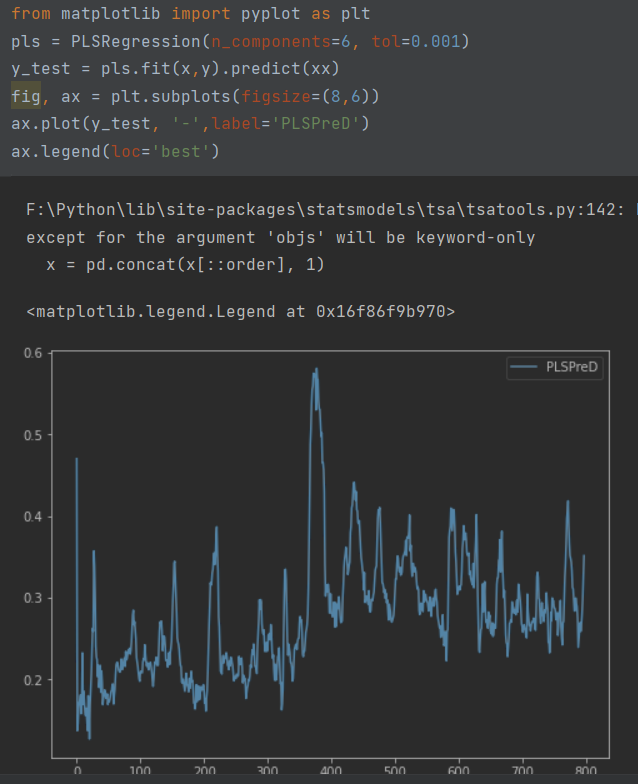
\includegraphics[width=0.5\textwidth]{images/PPPP.png}
  \caption{\lstinline{PLS}模型对测试集的拟合} 
\end{figure}

\subsection{多元线性回归}

在回归分析中,如果有两个或两个以上的自变量,就称为多元回归。
对于多元线性回归,或者可以称为多变量线性回归,我们认为各个特征和预测值之间是简单的加权
求和关系。这个假设在很多时候很牵强,但确实也在一些应用中性能不错。

作为机器学习入门而言,它相较于一元线性回归复杂一些,更加接近能够真实工作的机器学习应
用。因为在实际中,机器学习几乎总是处理多变量或者多特征。事实上,一种现象常常是与多个因
素相联系的,由多个自变量的最优组合共同来预测或估计因变量,比只用一个自变量进行预测或估计
更有效,更符合实际。因此多元线性回归比一元线性回归的实用意义更大。

将所有变量包括因变量都先转化为标准分,再进行线性回归,此时得到的回归系数就能反映对应自
变量的重要程度。这时的回归方程称为标准回归方程,回归系数称为标准回归系数,表示如下:

$$
Z_{y}=\beta_{1} Z \cdot 1+\beta_{2} Z \cdot 2+\ldots+\beta_{k} Z \cdot k
$$

由于都化成了标准分,所以就不再有常数项a了,因为各自变量都取平均水平时,因变量也
应该取平均水平,而平均水平正好对应标准分0,当等式两端的变量都取 0 时,常数项也就为0了。

建立多元线性回归模型时,为了保证回归模型具有优良的解释能力和预测效果,应首先注意自变量的选择,其准则是:

\begin{enumerate}
  \item 自变量对因变量必须有显著的影响,并呈密切的线性相关
  \item 自变量与因变量之间的线性相关必须是真实的,而不是形式上的
  \item 自变量之间应具有一定的互斥性,即自变量之间的相关程度不应高于自变量与因变量之间的相关程度
  \item 自变量应具有完整的统计数据,其预测值容易确定
\end{enumerate}

多元回归模型自变量的选择可以利用变量之间的相关矩阵来解决模型的参数估计,同一元线性
回归方程一样,也是在要求误差平方和($\sum e_i$)为最小的前提下,用最小二乘法求解参数。

导入\lstinline{linear_model}模块,然后创建一个线性模型\lstinline{linear_model.LinearRegression},该线
性回归模型创建有几个参数:

\begin{enumerate}
  \item \lstinline{fit_intercept}:\lstinline{bool}量,选择是否需要计算截距,默认为\lstinline{True},如果中心化了的数据可以选择\lstinline{false}
  \item \lstinline{normalize}:\lstinline{bool}量,选择是否需要标准化(中心化),默认为\lstinline{false},和参数\lstinline{fit_intercept}有关,自行思考
  \item \lstinline{copy_x}:\lstinline{bool}量,选择是否幅值X数据,默认\lstinline{True},如果否,可能会因为中心化把X数据覆盖
  \item \lstinline{n_job}:\lstinline{int}量,选择几核用于计算,默认1,-1表示全速运行
\end{enumerate}

\begin{lstlisting}[language=Python]
#定义线性回归模型
def test_LinearRegrssion():
    import parameters
    import load_data
    from sklearn import linear_model
    import pandas as pd 
    path = parameters.G_DataPath
    x_train, y_train, x_test = load_data.load_train_data(path)
    print(x_train.shape)
    regr = linear_model.LinearRegression()
    #训练数据
    regr.fit(x_train,y_train)
    #权重向量即为每个特征的相关系数
    print('Coefficients:%s,intercept %.2f' % (regr.coef_, regr.intercept_))
    y_test=regr.predict(x_test)
    data = pd.DataFrame(y_test)
    writer = pd.ExcelWriter('test.xlsx')
    # ‘page_1’是写入excel的sheet名
    data.to_excel(writer, 'page_1', float_format='%.5f')       
    writer.save()
    writer.close()
\end{lstlisting}

最终系统中测试结果\lstinline{0.1901},但由于模型自身限制,无法进一步优化,选择尝试其他模型。

\subsection{逻辑回归}

逻辑回归本质上是线性回归,只是在特征到结果的映射中加入了一层函数映射,即先把特征线性求和,然后使
用函数$g(z)$将最为假设函数来预测。$g(z)$可以将连续值映射到0到1之间。线性回归模型的表达式带入$g(z)$,就得到逻辑回归的表达式:

$$
h_{\theta}(x)=g\left(\theta^{T} x\right)=\frac{1}{1+e^{-\theta^{T} x}}
$$

\lstinline{Logistic}回归实质:发生概率除以没有发生概率再取对数。就是这个不太繁琐的变换改变了取值区间的
矛盾和因变量自变量间的曲线关系。究其原因,是发生和未发生的概率成为了比值 ,这个比值就是一
个缓冲,将取值范围扩大,再进行对数变换,整个因变量改变。不仅如此,这种变换往往使得因变量和
自变量之间呈线性关系,这是根据大量实践而总结。所以,\lstinline{Logistic}回归从根本上解决因变量要不是连
续变量怎么办的问题。还有,\lstinline{Logistic}应用广泛的原因是许多现实问题跟它的模型吻合。例如一件事情
是否发生跟其他数值型自变量的关系。

多项式回归优化逻辑回归的思路和线性回归的思路以及优化算法是一致的,它是在逻辑回归的基础上在原来的数据
集维度特征上增加一些另外的多项式特征,使得原始数据集的维度增加,然后基于升维后的数据集
用逻辑回归的思路进行求解,从而得到相应的预测结果和各项的系数。

\begin{lstlisting}[language=Python]
#使用多项式回归对sklearn的逻辑回归进行优化
#效果不佳
from sklearn.linear_model import LogisticRegression as LR
from sklearn.datasets import load_breast_cancer
import matplotlib.pyplot as plt
from sklearn.model_selection import train_test_split
from sklearn.metrics import accuracy_score#精确性分数
from sklearn import linear_model
import pandas as pd 
from sklearn.linear_model import LogisticRegression
from sklearn.preprocessing import PolynomialFeatures
from sklearn.metrics import r2_score
from sklearn.model_selection import train_test_split
import numpy as np
from sklearn.preprocessing import MinMaxScaler
x_train=np.loadtxt('train_modify.txt',dtype=np.float64)
y_train=np.loadtxt('output_modify.txt',dtype=np.float64)
x_test=np.loadtxt('test_modify.txt',dtype=np.float64)
# 归一化处理   
mm = MinMaxScaler()
x_train = mm.fit_transform(x_train)
x_test = mm.fit_transform(x_test)
poly = PolynomialFeatures(degree=2)

print('训练集的维度:',x_train.shape)
x_train_poly = poly.fit_transform(x_train)
print('扩展后训练集的维度:',x_train_poly.shape)
lr = LogisticRegression(penalty='l2',max_iter=10000,tol=1e-20)# 逻辑回归
lr.fit(x_train,y_train.astype(str))
x_test_poly = poly.fit_transform(x_test) 
# 多测试集进行扩展,为了进行检测与分数预测
# penalty:惩罚项,默认为l2
# max_iter: 最大迭代次数
# tol:停止求解的标准,float类型,默认为1e-4。就是求解到多少的时候,停止,认为已经求出最优解
y_test = lr.predict(x_test)
\end{lstlisting}

从提交结果来看,不管是否扩展数据维度逻辑回归的效果都不太理想,逻辑回归更适用于分类任务,对于该预测任务的时序信息还有特征利用都不是太好,而且我们想要的预测值是连续值,这也导致了预测效果不佳。

可见不同的任务应该从原理出发选择合适的模型,不合适的模型不会带来理想的结果。


\subsection{支持向量回归(SVR)}

\lstinline{SVR}全称是\lstinline{support vector regression},
是\lstinline{SVM}(支持向量机\lstinline{support vector machine})对回归问题的
一种运用。所以在介绍\lstinline{SVR}之前,我们先简单的来了解一下什么是\lstinline{SVM}。

\lstinline{SVM}与\lstinline{logistic}分类器类似,也是一种二类分类模型,其基本模型定义为特
征空间上的间隔最大的线性分类器,其学习策略便是间隔最大化,最终可转化为一个凸二次规划问题的求解。

对于下面一个数据集,有两类分别使用$×$和$○$来表示。那么我们想要找到一条曲线来
区分这两类。可想而知,这样的曲线存在无数条,如何找到那一条最优的曲线呢?那就是要找到
间隔(Gap)最大的那一条曲线,然后我们就可以根据这条曲线来分类了。而这条曲线
,我们称为超平面。图中加粗的$×$与$○$,我们则称这些向量为支持向量。

\begin{figure}[H]
  \centering
  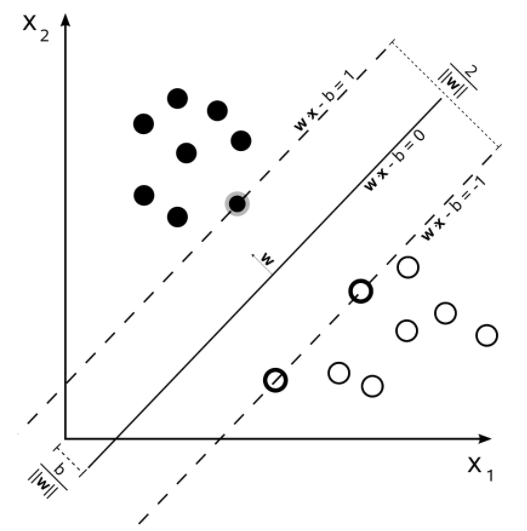
\includegraphics[width=0.5\textwidth]{images/SVM.png}
  \caption{\lstinline{SVM}超平面原理图} 
\end{figure}

而实际上,我们很少会遇到上面的情况,能直接使用一条直线将数据分类,更多的时候,数据无法通过直线来分类。比如下面这种情况:

\begin{figure}[H]
  \centering
  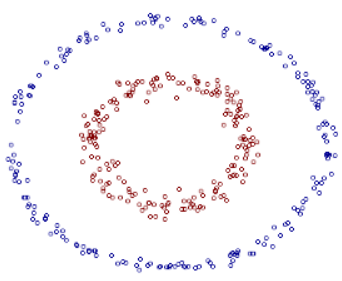
\includegraphics[width=0.5\textwidth]{images/SSS.png}
  \caption{无法通过实现分类的数据} 
\end{figure}

既然在二维上该数据无法使用线性分类,那我们就将数据映射到更高维上,在高维上构造超平面,从而完成分类。

\begin{figure}[H]
  \centering
  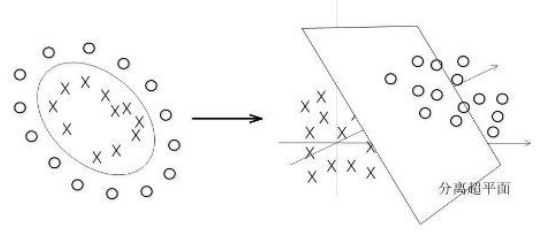
\includegraphics[width=0.5\textwidth]{images/SS.png}
  \caption{\lstinline{SVM}映射到更高维实现数据划分} 
\end{figure}

所以对于非线性的模型,我们需要:

\begin{enumerate}
  \item 使用非线性映射将数据投影至特征空间
  \item 在特征空间使用线性分类器
\end{enumerate}

但是我们在映射时,就会发现当变量增多时,映射到高维空间的
维度是呈指数增长的,计算起来十分困难,这时候就需要核函数(\lstinline{kernel function})了。核函数也是将特征从低维到高维进行转换,但
是它是先在低维上进行计算,实际的分类效果表现在高维上。这样,我们就避免了在高维上复杂的计算,仍得到相同的结果。

一些常用的核函数:

\begin{enumerate}
  \item 多项式核
  \item 高斯核
  \item 线性核
\end{enumerate}

我们知道,最简单的线性回归模型是要找出一条曲线使得残差最小。
同样的,\lstinline{SVR}也是要找出一个超平面,使得所有数据到这个超平面的距离最小。

\begin{figure}[H]
  \centering
  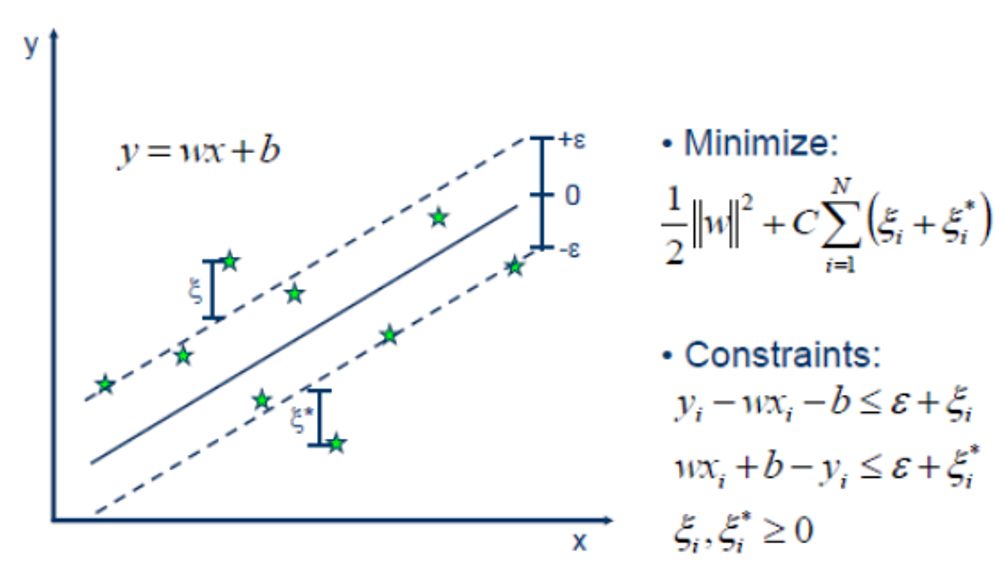
\includegraphics[width=0.5\textwidth]{images/SVR.png}
  \caption{\lstinline{SVR}基本原理} 
\end{figure}

如上文所述,\lstinline{SVR}是\lstinline{SVM}的一种运用,基本的思路是一致,除
了一些细微的区别。使用\lstinline{SVR}作回归分析,与\lstinline{SVM}一样,我们需要找到
一个超平面,不同的是:在\lstinline{SVM}中我们要找出一个间隔(gap)最大的超平面,而在\lstinline{SVR},我们
定义一个$\varepsilon$,如上图所示,定义虚线内区域的数据点的残差为$0$,而虚线区域外的数
据点(支持向量)到虚线的边界的距离为残差($\zeta$)。与线性模型类似,我们希望这些
残差($\zeta$)最小。所以大致上来说,\lstinline{SVR}就是要找出一个最佳的
条状区域($2\varepsilon$宽度),再对区域外的点进行回归。

\begin{figure}[H]
  \centering
  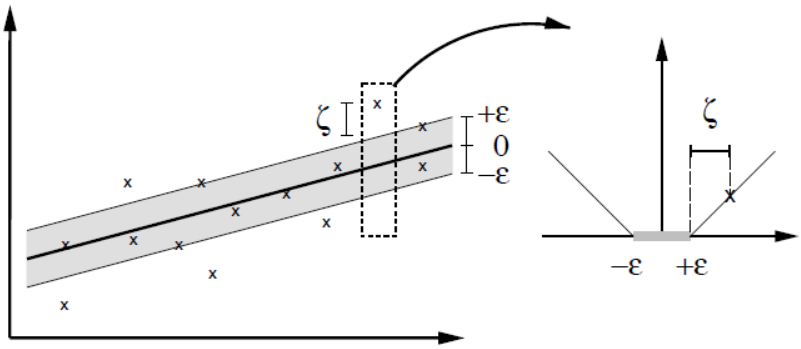
\includegraphics[width=0.5\textwidth]{images/SR.png}
  \caption{\lstinline{SVR}基本原理} 
\end{figure}

\begin{lstlisting}[language=Python]
from matplotlib import pyplot as plt
from sklearn.svm import SVR
import statsmodels.api as sm
svr = SVR()
x = data_train[['A','B','C','D','E','F','G']]
y = data_output[['Y']]
x=sm.add_constant(x)
y_fitted = svr.fit(x,y).predict(x)
\end{lstlisting}

我们这里还是使用\lstinline{sklearn.svm import SVR}的方式来简单
调用\lstinline{SVR}的工具包。能看到,\lstinline{SVR}的回归结果和\lstinline{OLS}与\lstinline{PLS}还是某种程度上相似的。为了防止过
拟合,它不会注重个别过高或过低点,最终给出一个相对中肯的模型。

\begin{figure}[H]
  \centering
  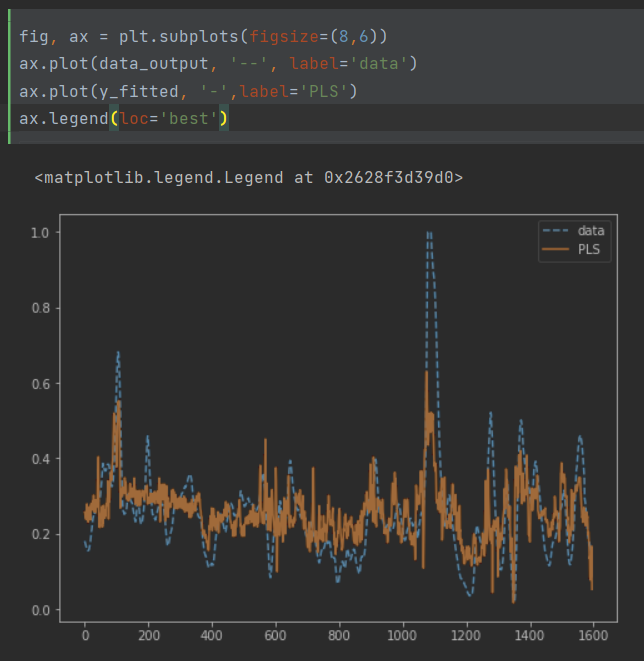
\includegraphics[width=0.5\textwidth]{images/RRR.png}
  \caption{\lstinline{SVR}对于验证集的拟合} 
\end{figure}

\begin{figure}[H]
  \centering
  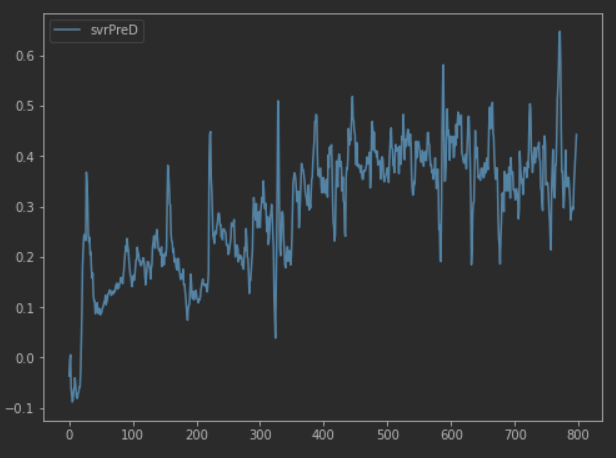
\includegraphics[width=0.5\textwidth]{images/RR.png}
  \caption{\lstinline{SVR}对于测试集的拟合} 
\end{figure}

但是,\lstinline{SVR}回归的结果在预测集上的结果显示不加,其震动幅度
比较大,而且结果并没有很好地刻画原数据集的特征,体现在数据不断
上升、抖动大这种明显的预测问题。更重要的是,\lstinline{SVR}也无法解决数据存在时
序相关的问题。最终我们发现\lstinline{SVR}预测结果的\lstinline{RMSE}的分数没有前面的几种方
法低,因此还是要考虑更换新的算法。

\subsection{随机森林}

回归随机森林作为一种机器学习和数据分析领域常用且有效的算法,很值得我们在本题中使用。

随机森林属于\lstinline{Bagging}类算法,而\lstinline{Bagging} 又属于集成学习一种方法。集成学习的大致思
路是训练多个弱模型打包起来组成一个强模型,强模型的性能要比单个弱模型好很多
(三个臭皮匠顶一个诸葛亮。注意:这里的弱和强是相对的),其中的弱模型可以是
决策树、\lstinline{SVM}等模型,在随机森林中,弱模型选用决策树。

随机森林本质上就是使用多棵树的决策结果来代替多棵树,起到一个很好的模型拟合效果。

在训练阶段,随机森林使用\lstinline{bootstrap}采样从输入训练数据集中采集多个不同的子训练数据
集来依次训练多个不同决策树;在预测阶段,随机森林将内部多个决策树的预测结果取平均得到最终的结果。
一般来说,随机森林的实现有如下过程:

\begin{enumerate}
  \item 模型训练
  \item 模型数据预测
  \item 计算\lstinline{feature importance}
\end{enumerate}

我们代码中选用的还是\lstinline{sklearn}库为我们准备好的随机森林模型。

\begin{lstlisting}[language=Python]
from sklearn import ensemble
random_forest_regressor = ensemble.RandomForestRegressor()
\end{lstlisting}

在训练二叉决策树模型的时候需要考虑怎样选择切分变量(特征)、切分点以及怎样衡量一个切分变量、切分点的好坏。

针对于切分变量和切分点的选择,一般我们采用穷举法,即遍历每个特征和每个特征的所有取值,最后从中找出最好
的切分变量和切分点;针对于切分变量和切分点的好坏,一般以切分后节点的不纯
度来衡量,即各个子节点不纯度的加权和 $G\left(x_{\{i\}}, v_{\{i j\}}\right)$。

计算公式如下:

$$
G\left(x_{i}, v_{i j}\right)=\frac{n_{1 \mathrm{eft}}}{N_{s}} H\left(X_{1 \mathrm{eft}}\right)+\frac{n_{\text {right }}}{N_{s}} H\left(X_{\text {right }}\right)
$$

其中,$x_i$是某一个切分变量,$v_{i}$ 为切分变量
的一个切分值,$n_left$、$n_right$,$N_s$分别为切
分后左子节点的训练样本个数、右子节点的训练样本
个数以及当前节点所有训练样本个数。$X_{left}$ 和$X_{right}$ 为左右子节点的
训练样本集合,$H(X)$为衡量节点不纯度的函数(\lstinline{impurity function/criterion}),分类和回归任务
一般采用不同的不纯度函数,在分类和回归常采用的不纯度函数有以下四种:

\begin{enumerate}
  \item 基尼系数:$\displaystyle \boldsymbol{H}\left(X_{m}\right)=\sum_{k} p_{m k}\left(1-p_{m k}\right)$
  \item 信息熵:$\displaystyle \boldsymbol{H}\left(\boldsymbol{X}_{\mathrm{m}}\right)=-\sum_{k} p_{m k} \log \left(p_{m k}\right)$
  \item \lstinline{MSE}:$\displaystyle \boldsymbol{H}\left(\boldsymbol{X}_{\boldsymbol{m}}\right)=\frac{1}{N_{m}} \sum_{i \in N_{\mathrm{m}}}\left(y-\overline{y_{m}}\right)^{2}$
  \item \lstinline{MAE}:$\displaystyle \boldsymbol{H X}_{\mathrm{m}}=\frac{1}{N_{m}} \sum_{i \in N_{\mathrm{m}}}\left|y-\overline{y_{m}}\right|$
\end{enumerate}

我们在实现的时候要注意如下几个点:

\begin{enumerate}
  \item \lstinline{Gini}系数只适用于分类任务,$X_m$为当前节点的训练样本集合,$p_{mk}$为当前节点训练样本中目标变量取值${{\mathrm{K}}}\left(p_{m k}=\frac{N_{m k}}{N_{m}}\right)$出现的概率。
  \item 信息熵只适用于分类任务, 其他同(1)。
  \item \lstinline{MSE}只适用于回归任务,$\overline{y_m }$ ̅为当前节点样本目标变量的平均值。
  \item \lstinline{MAE}只适用于回归任务,$\overline{y_m }$ ̅为当前节点样本目标变量的平均值。
  \item 在\lstinline{sklearn}内部
  ,\lstinline{DecisionTreeClassifier}, \lstinline{RandomForestClassifier}等基于决策树的分类模型默认使用
  \lstinline{Gini}作为\lstinline{impurity function},也可通过\lstinline{criterion}参数指
  定为\lstinline{entropy};而\lstinline{DecisionTreeRegressor}, \lstinline{RandomForestRegressor}等
  基于决策树的回归模型默认使用\lstinline{MSE}作为\lstinline{impurity function},也可通过\lstinline{criterion}参数指定为\lstinline{MAE}。
\end{enumerate}

决策树中某一节点的训练过程在数学等价于下面优化问题:

$$
\left(x^{*}, v^{*}\right)=\operatorname{argmin}_{x, v} G\left(x_{i}, v_{i j}\right)
$$

即寻找$G$最小的切分变量和切分点。
我们用\lstinline{MSE}实现的时候,则针对某个切分点,有如下的公式:

$$
G(x, v)=\frac{1}{N_{s}}\left(\sum_{y_{i} \in X_{\text {left }}}\left(y_{i}-\overline{y_{\text {left }}}\right)^{2}+\sum_{y_{j} \in X_{\text {right }}}\left(y_{j}-\overline{y_{\text {right }}}\right)^{2}\right)
$$

随机森林的实现较为复杂,要先对数据进行预处理,然后进行标注,最后才能输入我们的\lstinline{sklearn}库函数中:

\begin{lstlisting}[language=Python]
from sklearn.model_selection import train_test_split
from sklearn.model_selection import GridSearchCV
#data_train(全部数据) output(全部目标值)
#X_train训练集(全部特征) Y_train训练集的目标值
#test同理。
# 这里没有设置random
X_train, X_test, Y_train, Y_test = train_test_split(data_train,output, test_size=0.2,shuffle=False) #这里训练集75%:测试集25%
import numpy as np
from sklearn import ensemble

random_forest_regressor = \
ensemble.RandomForestRegressor(criterion='poisson', \
max_features='sqrt', \
n_estimators=500)

x = data_train[['A','B','C','D','E','F','G']]
y_ori = data_output[['Y']]
y = []
for i in range(len(y_ori)):
    y.append(y_ori[y_ori.columns[0]][i])
print(np.shape(y))
L = random_forest_regressor.fit(x, y)
pred = L.predict(x)

# y_fitted, y
from sklearn import metrics
# data_pre = model.predict(X_test)
MSE = metrics.mean_squared_error(pred, y)
print("MSE  ->", MSE)
RMSE = metrics.mean_squared_error(pred, y)**0.5
print("RMSE ->", RMSE)


RF1 = random_forest_regressor.fit(X_train, Y_train)

from sklearn.metrics import mean_squared_error
Y_train_pred = RF1.predict(X_train)

Y_test_pred = RF1.predict(X_test)
Y_test = np.array(Y_test)
print(mean_squared_error(Y_train,Y_train_pred))
# 拟合
print(mean_squared_error(Y_test,Y_test_pred))
from matplotlib import pyplot as plt
fig1, ax1 = plt.subplots(figsize=(8,6))
ax1.plot(Y_train_pred, '--', label='RF1')
ax1.plot(Y_train, '-',label='Y_train')
ax1.legend(loc='best')

fig2, ax2 = plt.subplots(figsize=(8,6))
ax2.plot(Y_test_pred, '--',label='RF1')
ax2.plot(Y_test, '-', label='Y_test')
ax2.legend(loc='best')
\end{lstlisting}

\begin{figure}[H]
  \centering
  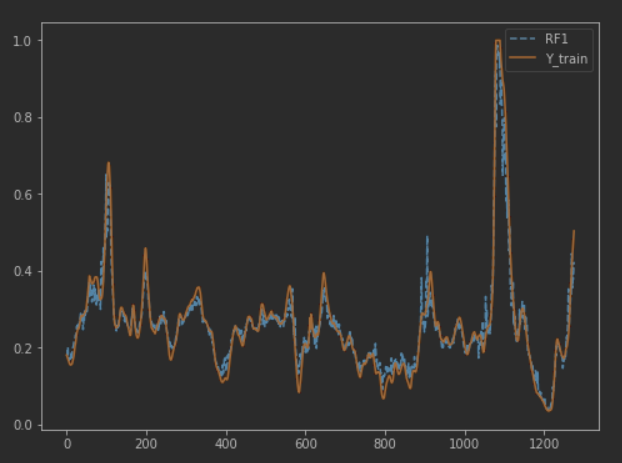
\includegraphics[width=0.5\textwidth]{images/FFFF.png}
  \caption{随机森林对于验证集的拟合} 
\end{figure}

能看到,随机森林抓取模型特征的能力非常的强,它几乎能满足所有训练值的点。如下图所示,但是值得一提的是,随机森林并不会有过强的过拟合现象
,因为它使用很多棵决策树来进行调整,而树的深度和树的数量是我们可以调整的,这也是我们的随机森林模型可以优化的地方。

预测代码编写如下:

\begin{lstlisting}[language=Python]
import numpy as np
from sklearn import ensemble
from matplotlib import pyplot as plt
import statsmodels.api as sm
from sklearn.model_selection import cross_val_score
x = data_train[['A','B','C','D','E','F','G']]
y_ori = data_output[['Y']]
y = []
for i in range(len(y_ori)):
    y.append(y_ori[y_ori.columns[0]][i])
print(np.shape(y))
# x=sm.add_constant(x)

random_forest_regressor = \
ensemble.RandomForestRegressor(criterion='poisson', \
max_features='sqrt', \
n_estimators=500)

print(np.shape(y))

RF = random_forest_regressor.fit(x, y)
y_fitted = RF.predict(x)
scores = cross_val_score(RF,x,y)
scores.mean()
\end{lstlisting}


\begin{figure}[H]
  \centering
  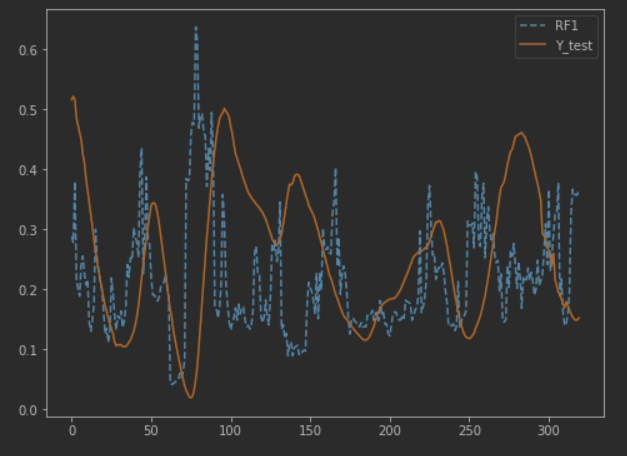
\includegraphics[width=0.5\textwidth]{images/FFFFF.png}
  \caption{随机森林对于测试集的拟合} 
\end{figure}

能看到,随机森林的模型在经过参数的调整后,已经基本能看到对测试集数据回归的趋势是大致正确的,在本地测试集测试时,\lstinline{RMSE}的值有了进一步的下降。

但是某种程度上来讲,它的某些特征抓取能力过强,还是有一些过拟合的现象发生。我们在调整了若干参数后,仍然可以看到它对于训练集的拟合还是过分准确,再考虑数据的时序性,这也导致我们不得不选择其他的方法。

\begin{figure}[H]
  \centering
  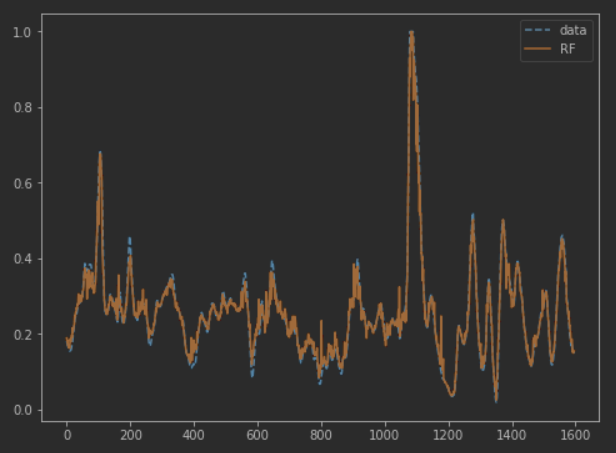
\includegraphics[width=0.5\textwidth]{images/FFFFFF.png}
  \caption{随机森林对于验证集的拟合(调参后)} 
\end{figure}

最后不得不说,尽管在我们本次数据上随机森林表现一般,但其实随机森林其实是一种很好的回归模型,在很多种场合都有广泛的应用。

\subsection{BP神经网络}

\subsubsection{算法介绍}

BP神经网络是一种按误差逆传播算法训练的多层前馈网络,是目前应用最广泛的神经
网络模型之一。BP网络能学习和存贮大量的 输入-输出模式映射关系,而无需事前揭示
描述这种映射关系的数学方程。它的学习规则是使用最速下降法,通过反向传播来不断
调整网络的权值和阈值,使网络的误差平方和最小。

多层感知器在如何获取隐层的权值的问题上遇到了瓶颈。既然我们无法直接得到隐层的权值
,能否先通过输出层得到输出结果和期望输出的误差来间接调整隐层的权值呢?
BP算法就是采用这样的思想设计出来的算法,它的基本思想是,学习过程由信号的
正向传播与误差的反向传播两个过程组成。

正向传播时,输入样本从输入层传入,经各隐层逐层处理后,传向输出层。若输出层的实际输出与期望的输出(教师信号)不符,则转入误差的反向传播阶段。

反向传播时,将输出以某种形式通过隐层向输入层逐层反传,并将误差分摊给各层的所有单元,从而获得各层单元的误差信号,此误差信号即作为修正各单元权值的依据。

\subsubsection{模型搭建}

该模型效果不佳,此处不多介绍,仅贴出\lstinline{matlab}代码。

\begin{lstlisting}[language=matlab]
%构造输出矩阵
s = length(trainl);
output = trainl;
%创建神经网络
net = newff( minmax(input) , [500 1], { 'logsig' 'purelin' } , 'traingdx' ); 
%设置训练参数
net.trainparam.show = 50;
net.trainparam.epochs = 1000;
net.trainparam.goal = 0.001;
net.trainParam.lr = 0.001;
%开始训练
net = train( net, input , output );
%测试数据归一化
testInput = tramnmx ( testd , minI, maxI );
%仿真
Y = sim( net , testInput )
\end{lstlisting}

\subsubsection{改进方向}

\begin{enumerate}
  \item 缺失值处理:缺失值处理上还需要多下些功夫,考虑尝试其他插值方法,比如k近邻算法。k近邻算法是在训练数据集中找到与该实例最邻近的K个实例。来了一个新的输入实例,我们算出该实例与每一个训练点的距离,然后找到前k个,这k个哪个类别数最多,我们就判断新的输入实例就是哪类。数据处理的好坏直接影响到了模型训练结果,本次建模过程中使用拉格朗日插值的建模效果远不如随机森林插值效果好。
  \item 考虑时滞性:虽然本次建模已经考虑了前一段时间特征对当前时间点的影响,但是没有单独分析每个变量的时滞性,有些变量在实际意义上相对于其他变量可能具有时滞性,简单的将整体平移无法利用这一点,需要单独处理变量。
  \item 模型结合:将多种模型的预测结果更好地结合起来分析,考虑多模型融合,发挥各个模型的长处。
\end{enumerate}

\subsection{深度神经网络(DNN)}

除了经典的\lstinline{LSTM}模型,我们还进行了充分的尝试,首先想到使用深度神经网络进行模型预测。

深度神经网络具有多层隐层神经元,能够从数据中提取更为抽象的特征,已得到具有较高准确率、较强泛化性的模型
以预测未来的脱丁烷塔温度。我们的想法是以二维数组作为模型输入\lstinline{(weight, height)},其中宽度表示
时间序列,长度表示每一个时刻的全部维度特征。再将处理好的数据传入模型进行训练,之后在\lstinline{RMSE}
标准下进行模型评估。

\subsubsection{数据预处理}

起初,我们使用相对简单的预处理方法,使用三个时刻的数据预测一个温度值,此时模型输入的数据形状为
\lstinline{(21,)},但是为了放大数据信息,我将数据形状扩展为\lstinline{(21,21)}。同样为了进行
更多的尝试,我还将数据进一步扩展为\lstinline{(42,42)},以图片格式输出如下。

\begin{figure}[H]
  \centering
  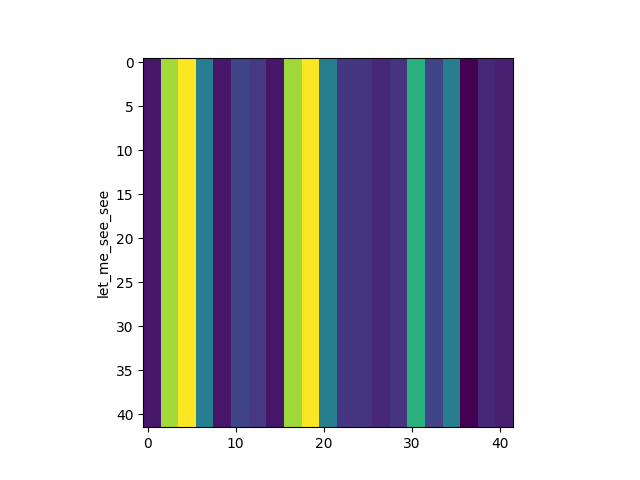
\includegraphics[width=0.5\textwidth]{images/4242.png}
  \caption{形状为\lstinline{(42,42)}的模型输入数据} 
\end{figure}

后来也有尝试过使用不仅三个时刻的数据,比如使用之前5个时刻,之前10个时刻等,最多使用到了之前20个时刻,
但是本地检验的模型准确度仍然是前三个时刻的最高,可能是因为噪声对的占比增加导致的。

\subsubsection{模型搭建}

我们的想法是,使用$2 \sim 3$层网络应该足够进行预测,因为本项目的数据相比于图片数据,
维度明显更少,应该不需要进行很复杂的特征提取。但是在实际操作中,$2\~3$层的模型
收敛效果不好,严重欠拟合。于是我们逐渐增加深度,最终的模型如下:

\begin{lstlisting}[language=Python]
dropout_param = 0.2
model = Sequential()
model.add(Dense(128, input_shape=(width, height), kernel_initializer='normal', activation='relu'))
model.add(Dropout(dropout_param))
model.add(Dense(256, kernel_initializer='normal', activation='relu'))
model.add(Dropout(dropout_param))
model.add(Dense(512, kernel_initializer='normal', activation='relu'))
model.add(Dropout(dropout_param))
model.add(Dense(1024, kernel_initializer='normal', activation='relu'))
model.add(Dropout(dropout_param))
model.add(Dense(2048, kernel_initializer='normal', activation='relu'))
model.add(Dropout(dropout_param))
model.add(Dense(2048, kernel_initializer='normal', activation='relu'))
model.add(Dropout(dropout_param))
model.add(Dense(1024, kernel_initializer='normal', activation='relu'))
model.add(Dropout(dropout_param))
model.add(Dense(1024, kernel_initializer='normal', activation='relu'))
model.add(Dropout(dropout_param))
model.add(Dense(512, kernel_initializer='normal', activation='relu'))
model.add(Dropout(dropout_param))
model.add(Dense(256, kernel_initializer='normal', activation='relu'))
model.add(Dropout(dropout_param))
model.add(Dense(128, kernel_initializer='normal', activation='relu'))
model.add(Dropout(dropout_param))
model.add(Dense(1, kernel_initializer='normal', activation='linear'))
\end{lstlisting}

\subsubsection{模型训练}

下图是我组认为收敛效果较优的两次训练:

\begin{figure}[H]
  \centering
  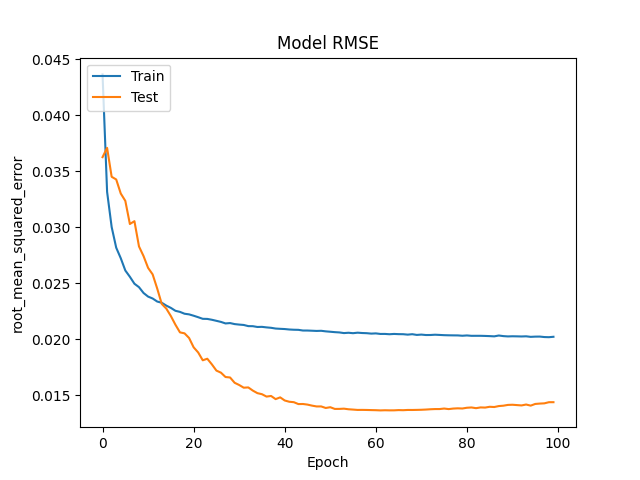
\includegraphics[width=0.5\textwidth]{images/RMSE_NN.png}
  \caption{\lstinline{DNN}迭代100次\lstinline{Loss}曲线} 
\end{figure}

\begin{figure}[H]
  \centering
  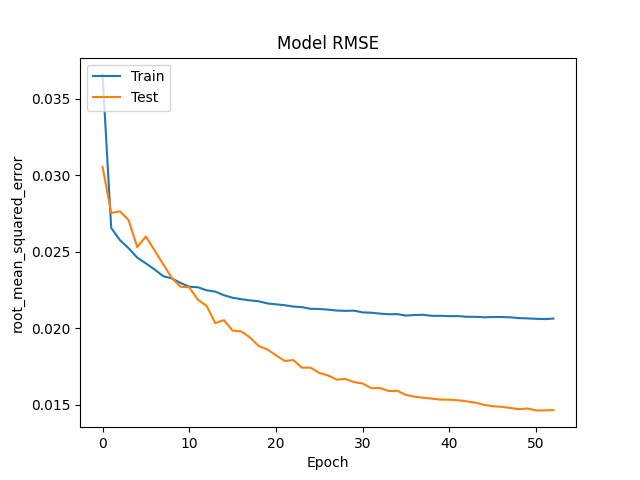
\includegraphics[width=0.5\textwidth]{images/RMSE_NN_1.png}
  \caption{\lstinline{DNN}迭代50次\lstinline{Loss}曲线} 
\end{figure}

图中可以看到,在训练过程中,\lstinline{Test}的\lstinline{Loss}一直明显低于\lstinline{Train}。我们认为模
型出现了比较严重的欠拟合,但是当我们继续复杂化网络时,却发现模型预测逐渐趋于恒值,而且\lstinline{Test}的\lstinline{Loss}
依旧明显低于\lstinline{Train}。

\subsubsection{模型评估}

在本地训练时,\lstinline{DNN}的\lstinline{RMSE}表现为0.147,但是提交的时候成绩是0.198,本地
测试的拟合图如下。

\begin{figure}[H]
  \centering
  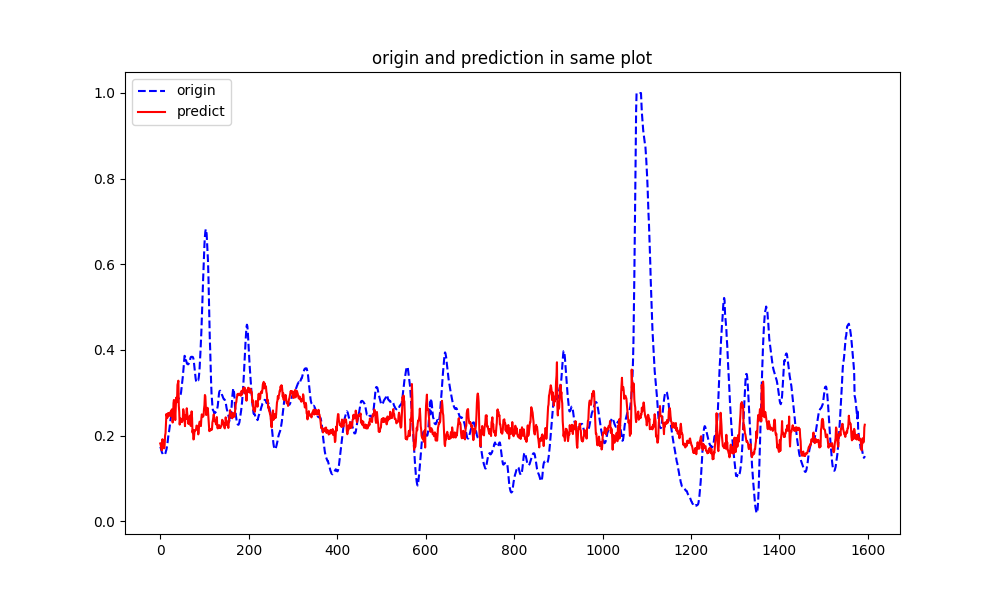
\includegraphics[width=0.5\textwidth]{images/NN_PRED.png}
  \caption{\lstinline{DNN}本地测试曲线} 
\end{figure}

和普通\lstinline{OLS}、\lstinline{pls}的跑分差不多,并没有体现出神经网络的优势,我们看到这个结果
还是比较沮丧的,因为我们认为,伸进网络虽然不能从数据中直接提取时序特征,但是能够很好的提取出
空间特征,于是我们想通过在数据预处理的过程中手动引入时序特征,采取之前几个时刻的数据一起预测
当前时刻的温度正是为了这个。

\subsection{卷积神经网络(CNN)}

类似上述\lstinline{DNN}的方法,我们还使用了卷积神经网络进行温度预测的尝试。
相比于普通深度神经网络,\lstinline{CNN}能够更有效的提取空间特征,而且可以通过
合理地设置\lstinline{dropout()}参数以避免过拟合等问题。

\subsubsection{数据预处理}

类似于上述\lstinline{DNN}的预处理方法,我们尝试通过数据预处理在模型输入数据中人为引入
时序信息,即通过综合使用之前几个时刻的数据进行温度预测。

\subsubsection{模型搭建}

起初我们仅使用了5层左右的伸进网络模型,但是模型收敛效果不好,于是我们逐渐复杂化模型,层架神经网络层数以及
隐层神经元的数量,最终模型如下:

\begin{lstlisting}[language=Python]
dropout_param = 0.2
model = Sequential()
model.add(Conv2D(filters=32, kernel_size=(2, 2), padding='same', data_format='channels_last', input_shape=(width, height, 1), activation='relu'))
model.add(MaxPooling2D(pool_size=(2, 2)))
model.add(Dropout(dropout_param))
model.add(Conv2D(filters=32, kernel_size=(2, 2), padding='same', data_format='channels_last', input_shape=(width, height, 1), activation='relu'))
model.add(MaxPooling2D(pool_size=(2, 2)))
model.add(Flatten())
model.add(Conv2D(filters=32, kernel_size=(2, 2), padding='same', data_format='channels_last', input_shape=(width, height, 1), activation='relu'))
model.add(MaxPooling2D(pool_size=(2, 2)))
model.add(Dropout(dropout_param))
model.add(Conv2D(filters=32, kernel_size=(2, 2), padding='same', data_format='channels_last', input_shape=(width, height, 1), activation='relu'))
model.add(MaxPooling2D(pool_size=(2, 2)))
model.add(Flatten())
model.add(Dropout(dropout_param))
model.add(Dense(256))
model.add(Activation('relu'))
model.add(Dropout(dropout_param))
model.add(Dense(128))
model.add(Activation('relu'))
model.add(Dropout(dropout_param))
model.add(Dense(1, activation='linear'))
\end{lstlisting}

\subsubsection{模型训练}

下面是我们认为效果比较优秀的一次训练\lstinline{log}信息:

\begin{figure}[H]
  \centering
  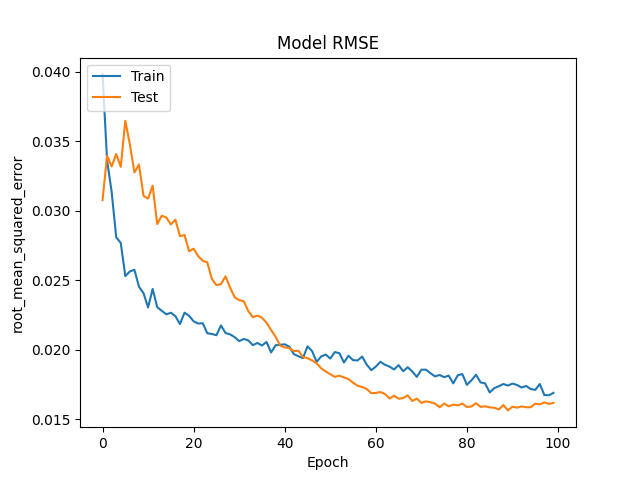
\includegraphics[width=0.5\textwidth]{images/RMSE_CNN.png}
  \caption{\lstinline{CNN}迭代100次\lstinline{Loss}曲线} 
\end{figure}

图中我们可以看到,\lstinline{Train}与\lstinline{Test}并没有出现很明显的分离,而是
一起在收敛,效果较好。

\subsubsection{模型评估}

在本地训练时,\lstinline{DNN}的\lstinline{RMSE}表现为0.133,但是提交的时候成绩是0.191。
成绩还是不能够令人满意。经分析后,我们认为有以下两点需要改进:

\begin{enumerate}
  \item 不能盲目地扩充数据量,应该精准地进行数据预处理
  ,有效地进行不同维度的组合,除去噪声较大的维度,保留有效特征,不要让与最终输出不相关的维度进入模型的训练。
  \item 时序特征的提取不够彻底,加入前几个时刻的数据虽然是在一定程度上为模型引入了时序特征,但是像\lstinline{DNN}以及、
  \lstinline{CNN}都是主要用来提取空间特征的模型,为了更加有效地提取时序特征,我们还是需要采用像\lstinline{LSTM}、\lstinline{RNN}
  、\lstinline{Transformer/Bert}之类的时序特征提取模型,或者进行两者的组合。
\end{enumerate}


\subsection{卷积自编码器(CAE)}

\subsubsection{设计初衷}

在别的课程大作业中,有使用过卷积自编码器进行数据特征的提取,并通过检验模型的数据再生成能力已验证数据中提取空间信息的有效性与合理性。
本次实验中数据量较少,想通过提取空间上的特征生成一些新数据,并以此提升原始训练数据的质量,以平衡噪声,突出数据中的有效特征。


\subsubsection{模型搭建}

本项目中使用的卷积自编码器模型如下:

\begin{lstlisting}[language=Python]
input_img = Input(shape=(width, height, 1))
x = Conv2D(16, (2, 2), activation='relu', padding='same')(input_img)
x = MaxPooling2D((2, 2), padding='same')(x)
x = Conv2D(8, (2, 2), activation='relu', padding='same')(x)
x = MaxPooling2D((2, 2), padding='same')(x)
x = Conv2D(8, (2, 2), activation='relu', padding='same')(x)
encoded = MaxPooling2D((2, 2), padding='same')(x)
x = Conv2D(8, (2, 2), activation='relu', padding='same')(encoded)
x = UpSampling2D((2, 2))(x)
x = Conv2D(8, (2, 2), activation='relu', padding='same')(x)
x = UpSampling2D((2, 2))(x)
x = Conv2D(16, (2, 2), activation='relu')(x)
x = UpSampling2D((2, 2))(x)
decoded = Conv2D(1, (2, 2), activation='sigmoid', padding='same')(x)
autoencoder = Model(input_img, decoded)
\end{lstlisting}

\subsubsection{模型分析}

\begin{enumerate}
  \item 使用自编码器后,我们更加意识到了在本项目中空间特征的局限性了,不得不说空间特征提取的再好,也很难得到
  较低的\lstinline{RMSE}损失值。
  \item 还是需要注重数据本身的不同维度特征之间的组合,因为从以上的实践中,我们意识到有些维度的特征对于最终的结果所能提供的信息是相对有限的,
  也存在一些维度噪声很大,甚至会起到反作用的情况。
\end{enumerate}


\subsection{强化学习(RL)}

强化学习强调如何基于环境而行动,以取得最大化的利益,是除了监督学习和非监督学习之外的第
三种基本的机器学习方法。与监督学习不同的是,强化学习不需要带标签的输入输出对,同
时也无需对非最优解的精确地纠正。其关注点在于寻找探索(对未知领域的)
和利用(对已有知识的)的平衡。

\begin{figure}[H]
  \centering
  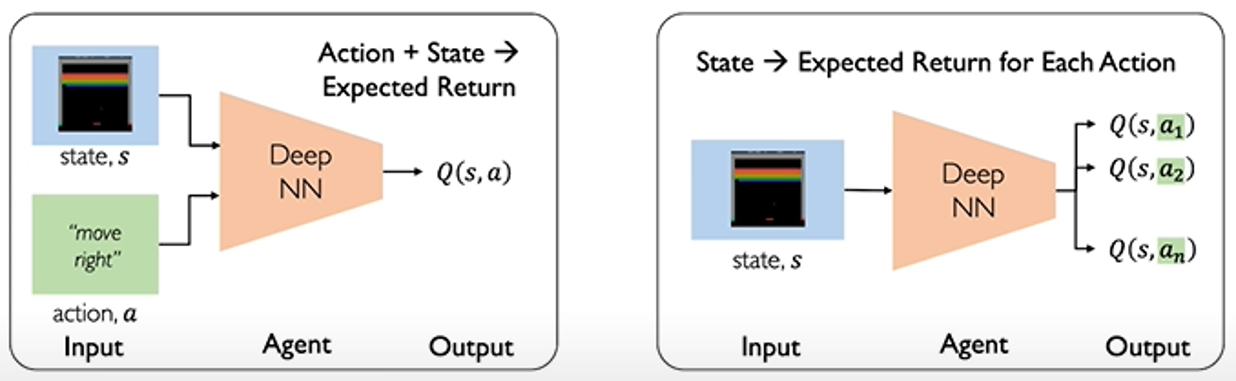
\includegraphics[width=0.5\textwidth]{images/RL.png}
  \caption{强化学习基本原理} 
\end{figure}

\begin{figure}[H]
  \centering
  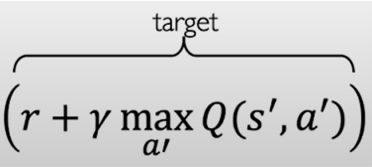
\includegraphics[width=0.3\textwidth]{images/RLL.png}
  \caption{强化学习优化目标} 
\end{figure}

我们也有尝试使用强化学习进行预测,并从网上学习了使用强化学习进行股票预测的代码,
但是对于强化学习模型的使用不熟悉,而且也不确定如何定义针对本温度预测项目的状态(state)
与操作(action),最终没有完全落地执行。

\subsection{循环神经网络(RNN)与LSTM}

\subsubsection{模型介绍}

我们知道神经网络是一种很强大的拟合工具,它可以拟合任何函数,而且它学习时十分听话,投入产出比高。我们只要喂给它足够的训练数据,他就会变得越发强力,一眼看去它就仿佛一个带着魔法的黑盒子一般。在网络训练好之后,我们给它一个输入量,就可以得到想要的输出结果。下图是神经网络一个简单的示意图。

\begin{figure}[H]
  \centering
  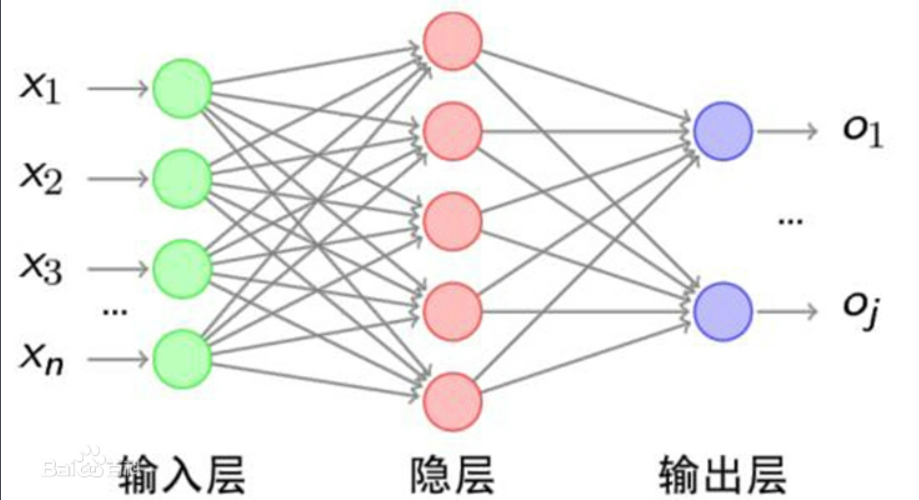
\includegraphics[width=0.5\textwidth]{images/NN.png}
  \caption{神经网络基本结构} 
\end{figure}

我们可以利用普通神经网络的强大特征抓取能力来做出一个人脸识别机器。其实这很容易,神经网络可以抓住许许多多我们忽略掉的特征,并且把这些特征以一组组隐藏层矩阵存储在自己的“脑海”里。它训练结束后,某种程度上比我们更善于辨识。

但是令人遗憾的是,我们在日常中遇到的问题可不止是对静态的目标进行识别。比方一段视频理论上可以按照时间分成许多帧的集合。然后我把这个视频交给 “CNN”,请它来分析一下视频中的人正在做什么以及接下来他可能会做什么这两个问题。它一定会去一帧一帧仔细翻看对比过后告诉我们一个答案:“说实话,我也不知道。我只能判断出这一叠叠照片中有个人。”

现实是这样的,我们强大的CNN虽然在对特征提取方面有着无与伦比的能力,但是这仅限于对一张静态的图片进行特征提取。CNN在接收到这段视频时,它不管这个视频里面第一秒和第二秒的情况有什么关联,在他眼中这两帧一点关系都没有,整个视频里面的每一帧之间也一点关系都没有。而我们看视频,除了看每一帧的画面,还要看一帧一帧之间的联系,比如我们可以给出以下的四张图片:

\begin{enumerate}
  \item 图片A——手在水杯前方。
  \item 图片B——手接触水杯。
  \item 图片C——手捏住水杯。
  \item 图片D——手和水杯一起起来了。
\end{enumerate}

如果是CNN,它会认为这四副图里面各有一只手和一个水杯。但是作为一个正常人,我们看到这四张图片会把它们一起理解为一个动作——“拿起水杯”。

显然我们不能再把这个问题交给CNN了。因为我们在观察图片的时候,发现了这几张
图片之间是有联系的,从而对这四张图片进行了某种整体的分析,得出了一个基于这种联系的结果,
而不是基于单纯某张图片的结果。相似地,我们在NLP(自然语言处理)中经常要分析一个句子,
而这个句子里面前一个词其实对后一个词的词性预测是有很大的影响的。这里给出这样的一个句子
——“我吃米饭。”这个句子我们可以清晰划分出来它的主谓宾结构来:“我”是名词,作为主语;“吃”是
动词,作为谓语;“米饭”是名词,作为宾语。很显然,动词后面接一个名词是再正常不过的事情了,换
句话说,当你在看到“我吃蒟蒻”(蒟蒻,一种魔芋)这种句子时,你虽然不知道蒟蒻是什么,但是你看到
它跟在了“吃”这个动词后面,那它很大可能就是一个名词,作为吃的宾语。对于一个成功机器来说,虽然它
第一次不知道“我吃米饭”中“米饭”的含义,但是它依旧可以通过其前一个字“吃”来推测得出“米饭”很大概率
会是一个名词。值得庆幸的是,这种成功的机器已经被我们设计出来了,它就是\lstinline{RNN(Recurrent Neural Network)}循环神经网络。

和简单的神经网络不同,RNN比CNN多了一个环节——它将上一个隐藏层的值经过处理后加到了下一个隐
藏层中,这样实际上就是将输出值作为输出值反馈了回来。反馈这个词我们应当是十分熟悉的,下
面两幅图给出了一个简单的RNN图示和我们自动控制理论中反馈回路的图示。

\begin{figure}[H]
  \centering
  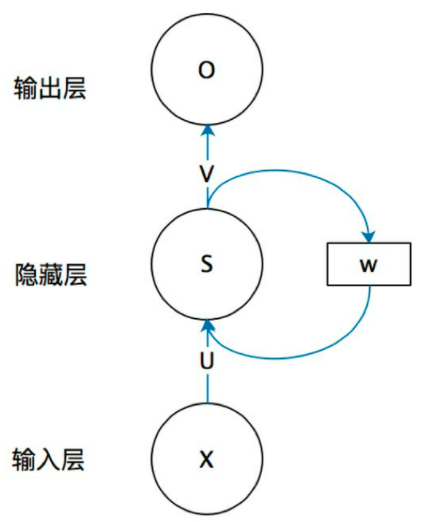
\includegraphics[width=0.3\textwidth]{images/RNN.png}
  \caption{RNN基本结构} 
\end{figure}

\begin{figure}[H]
  \centering
  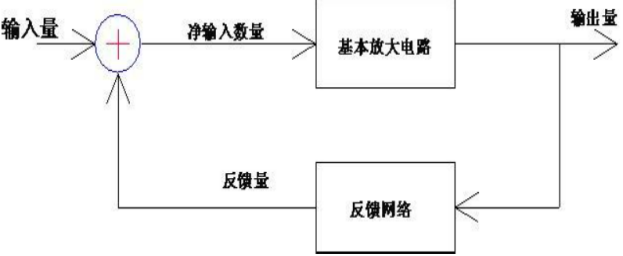
\includegraphics[width=0.5\textwidth]{images/FK.png}
  \caption{常见的电路反馈回路} 
\end{figure}

这里我们发现,两张图居然十分相似,都是在输出量前方引出一个反馈回路重新输送回去进行重新加工。在RNN对应的那张图中:

\begin{itemize}
  \item $X$是一个向量,代表着输入层。
  \item $S$是一个向量,代表着隐藏层,但是实际上$S$中可能有多个层,每个层都有多个节点,节点数量也和向量$S$的维度相同,这里只进行了最简单的表示。
  \item $O$是一个向量,它表示输出层。
  \item $U$很显然是从输入层到隐藏层的权重矩阵。
  \item $V$是从隐藏层到输出层的权重矩阵。
  \item $W$则是我们要重点研究的反馈环节,它有点类似于我们反馈回路中的反馈增益,那它实际上就是我们上一个隐藏层到这个隐藏层的权重矩阵。
\end{itemize}

其他层CNN也有,那我们不多赘述,具体在这里分析一下RNN比CNN多出来这一点本领究竟强在哪里,以及它为什么强大。

\begin{figure}[H]
  \centering
  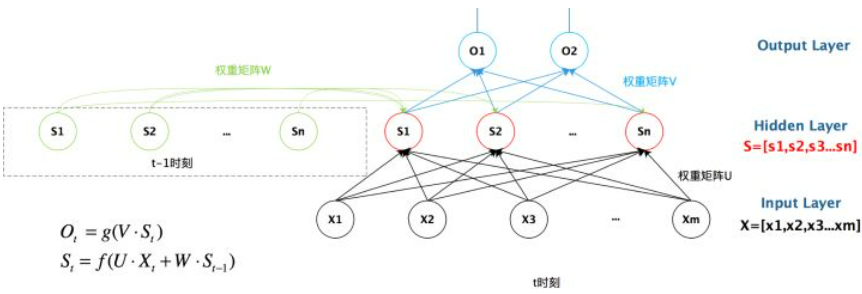
\includegraphics[width=0.5\textwidth]{images/FFKK.png}
  \caption{反馈环节基本结构} 
\end{figure}

上面这张图就对W反馈环节做了比较详细的解释,我们发现,在右边最下方首先是向量X的输入,然
后在权重矩阵U的作用下产生向量S,这里我们记为S1。然后下一个向量X2再输入时,首先是和权重矩
阵U的作用,这里还没结束,我们再把上一轮次的S1拿过来,给它乘以一个权重矩阵W,然后与UX2加在
一起,这样我们才算是得到了S2,以此类推。宏观来讲,我们就是通过这样的手段得到了来自于上一个
输入量X的信息,并且把二者的联系通过权重矩阵W给传递了下来。如图所示:

\begin{figure}[H]
  \centering
  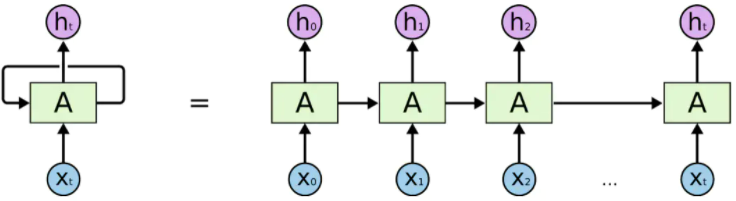
\includegraphics[width=0.5\textwidth]{images/WWW.png}
  \caption{RNN基本结构(展开)} 
\end{figure}

这里我们给出一个最基本的数学公式:


$$
\begin{aligned}
&O_{t}=g\left(V \cdot S_{t}\right) \\
&S_{t}=f\left(U \cdot X_{t}+W \cdot S_{t-1}\right)
\end{aligned}
$$

所以这就能解释为什么RNN可以自豪地告诉我们:“这段视频我判断他大概是在喝水。”没错,RNN还能被
广泛应用在时序信号的处理上,在音乐推荐、股市分析、疾病诊疗等方面RNN都有不俗的建树。

RNN理论上是可以将以前的信息与当前的任务进行连接,例如使用以前的视频帧来帮助理解当前帧。但是普通的R
NN网络在执行几次之后,它储存的记忆就会被新的信息所覆盖,导致产生某种程度的忘记,这是因为第一个向量S
的影响在每一层的权重矩阵W和每一层新变量X作用下,会被逐渐淡化,就好比是给一杯糖水里面不断添水,这杯糖水
的甜味也会越来越淡。一杯糖水当你刚加入一点水时,这杯水可能还会保持一定的甜度,例如我们在使用RNN语言模型
通过利用以前的文字来预测下一文字时,给出句子“天上有一朵(   )”,然后要求RNN来填空,RNN也许会不假思索就给出答
案“云”。因为地点状语“天上”和量词“朵”都可以帮助
我们做出判断,而且这个句子很短,读完这个句子,RNN尚存有短期记忆,那他自然有不错的表现。


\begin{figure}[H]
  \centering
  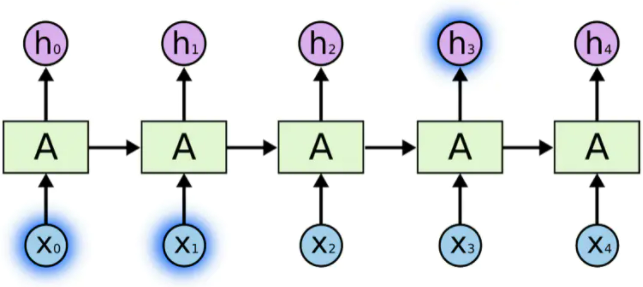
\includegraphics[width=0.5\textwidth]{images/XH.png}
  \caption{信息X和输出H离得很近} 
\end{figure}

同样一杯糖水,当你不断加入水,甚至还往里面加入果汁可乐奶茶等乱七八糟的东西
的时候,你也许很难辨认出这杯糖水来了,RNN也是如此,他短暂的记忆容不得这么庞杂
的信息,否则,他会逐渐“迷失自我”。考虑下面这句话:“我小时候在法国马赛长大,那
是一个美丽的城市。后来我离开了欧洲前往美国俄亥俄州的辛辛那提,我在那里我度过
了我的青年时光。我不是美国人,回到家后我仍旧只说(   )”根据上下文,这里显然填“
法语”。这种情况可能就是RNN难以应付的了,因为信息“法国马赛”实在是离最后一个填空
的地方太远了,RNN被后面大量多余的信息冲淡了记忆,最终可能会导致任务失败。


\begin{figure}[H]
  \centering
  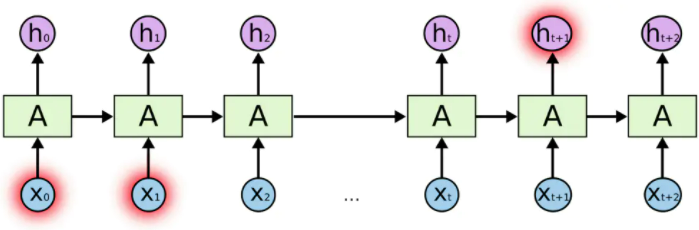
\includegraphics[width=0.5\textwidth]{images/XH2.png}
  \caption{信息X和输出H离得很远} 
\end{figure}

为了解决这个问题,两位研究人员Hochreiter和Schmidhuber在RNN的基础上,经过多年研究,发现了一位RNN的兄弟可以
解决这个信息冲淡的问题,于是我们就要介绍一下LSTM了。

LSTM(Long Short Term Memory networks)叫做长短期记忆网络,它解决
了这种信息冲淡的问题,它不同于简单的RNN,它的内部神经元内的反馈模块使
用了四个网络层而不是一个,如图所示。

\begin{figure}[H]
  \centering
  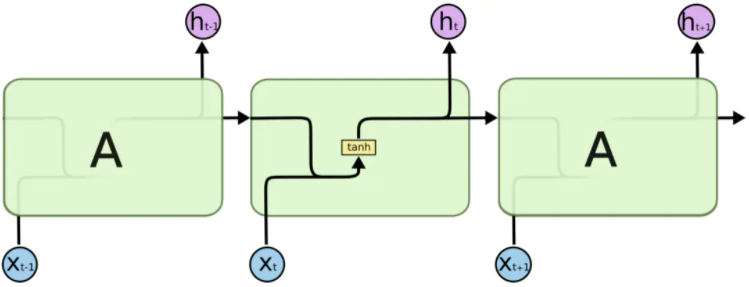
\includegraphics[width=0.5\textwidth]{images/LSTM.png}
  \caption{标准RNN只有一个tanh层} 
\end{figure}

\begin{figure}[H]
  \centering
  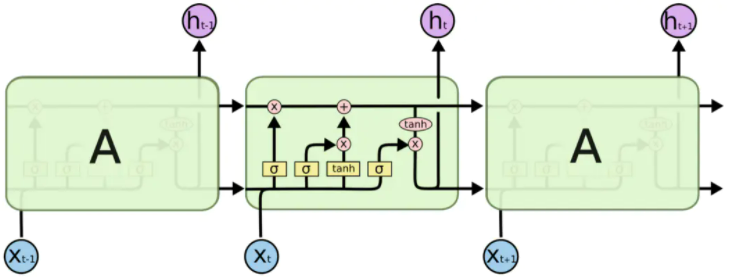
\includegraphics[width=0.5\textwidth]{images/LLLL.png}
  \caption{LSTM有复杂的4层} 
\end{figure}

图中黄色类似于CNN里的激活函数,粉色圆圈表示按位乘或相加操作,单箭头表
示数据流向,箭头合并表示向量的相加,箭头分叉表示向量从同一个值引出,
可以参考我们的方块图。

LSTM的核心是神经元的状态,用贯穿各个神经元的一条水平线表示,这就好比
是一个传送带,让LSTM学习到的信息在层与层之间滚动,输送到各个神经元中
,则每个神经元的输出就可以考虑到很久以前的信息了。可以说,LSTM是专门
为解决信息冲淡问题的。


要在两个层之间传递信息,那我们就不得不回答这些问题:

\begin{enumerate}
  \item 上一层哪些信息要留下?
  \item 上一层哪些信息要丢弃?
  \item 这一层哪些信息新输入了?
\end{enumerate}

LSTM是通过三个门环节来解决这三个问题的,它们分别被称为是忘记门、输入门和输出门。

忘记门,顾名思义,就是要决定上一层有多少信息我们要留下以及忘记的,
有点奈何桥的感觉了,不过它这里不是通过奈何桥而是通过了一个sigmoid
非线性函数。它把上一层输出Ht-1和这一层输入Xt都纳入考虑范围,然后
输出一个0-1之间的向量,这代表了上一个隐藏层信息Ct-1的继承比重。0表示
全部丢弃,1表示全部保留,给出公示如下:

\begin{figure}[H]
  \centering
  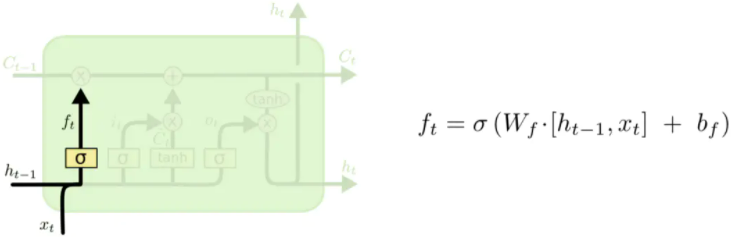
\includegraphics[width=0.5\textwidth]{images/FJ.png}
  \caption{LSTM忘记门} 
\end{figure}

输入门则利用Ht-1和Xt通过一个tanh函数来得到新的隐藏层信息Ct0,这些信
息可能被加入我们层之间的传送带中,但它这时还不是我们这层输出的真正
的Ct。与Ct0并行的还有一个sigmoid函数层,这个同样是为了对Ct进行比重的调整。

\begin{figure}[H]
  \centering
  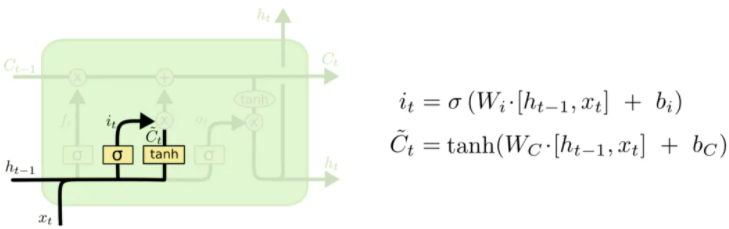
\includegraphics[width=0.5\textwidth]{images/SC.png}
  \caption{LSTM输出门} 
\end{figure}

这里通过忘记门和输入门后,我们对上一层的信息Ct-1和这一层的隐藏层信息Ct0进行合并,这样才得到隐藏层信息Ct。

\begin{figure}[H]
  \centering
  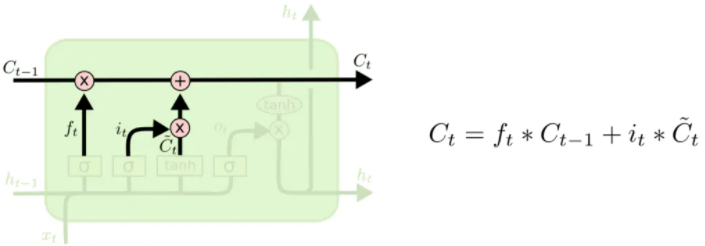
\includegraphics[width=0.5\textwidth]{images/TO.png}
  \caption{LSTM忘记门与输出门一起工作} 
\end{figure}

更新完隐藏层信息Ct后,我们再根据上一层和输出Ht-1和这一层的
输入Xt来得到这一层的输出,那么这里就通过我们的输出门,它实际上还
是一个sigmoid函数。并且还要再结合来自于本层隐藏层信息Ct的信息,最
终才能给出我们的整个LSTM最终输出。

可以看到,在整个隐藏层中,我们不再是简单地读取前一步的信息,而是
各部分之间打组合拳,层层递进才得到了我们最终的结果。LSTM脑海中就这样继
承了早期的记忆并且能一直在后面中保持应用。而我们不也应该如此吗,作为
学生,应当树立终身学习意识,就像LSTM一样,将之前所学的知识不断整合
,不断突破自己,才能拥有更光明的未来。

LSTM作为RNN的一种,在诞生后取得了很大的成就,在大部分的时序场景
也是能够使用并且取得了不错的性能的。LSTM还有很多很多的变种,比如
加入了“窥视孔连接”,使得所有门都能得到本层信息Ct或者上层信息Ct-1;
再比如在忘记门与输入门之间建立耦合,实际上是对Ct关于Ct-1和Ct0的比例
调整,我们有理由相信以后的研究成果也会更为丰富。

\subsubsection{迭代LSTM}

在我们本次的任务中,运用RNN和LSTM的手段来完成时间序列预测,则必须
要先实现将时间序列转换为python中的监督学习的问题。我们在这里用到
的深度学习库函数有如下:

\begin{lstlisting}[language=Python]
import copy
import numpy as np
import pandas as pd
\end{lstlisting}

在调用基本的库函数后,我们先对数据进行导入和初步的处理。特别强调
这里有一个keras中深复制和浅复制的概念,十分有趣。我们这里使用的是
深复制。随后就将其转化成我们的数据帧进行处理。

\begin{lstlisting}[language=Python]
# 读取数据
a=np.loadtxt('train_input.csv',dtype=np.float64)
b=np.loadtxt('output.txt',dtype=np.float64)
b = b[:,np.newaxis]
a[5] =(a[6]+a[5])/2
a = np.delete(a,6,axis=1)
#按行拼接,训练集输出也是信息
values=np.concatenate((a,b),axis=1)
#深复制而非浅复制,很有意思的
data = copy.deepcopy(values)
data = pd.DataFrame(data)
\end{lstlisting}

然后我们构建监督数据集\lstinline{series_to_supervised(data, n_in, n_out)}函数,具体内容见后文。

\begin{lstlisting}[language=Python]
def series_to_supervised(data, n_in, n_out):
    df = pd.DataFrame(data)
    n_vars = df.shape[1]  # n_vars 列数
    cols, names = list(), list()
    
    # 时间间隔跨度, 时间点个数,共 n_in 个
    # 首先添加当前时刻之前的时间点
    for i in range(n_in - 1, 0, -1):
        cols.append(df.shift(i))
        names += [('var%d(t-%d)' % (j + 1, i)) for j in range(n_vars)]
    # 然后添加当前时刻
    cols.append(df)
    names += [('var%d(t)' % (j + 1)) for j in range(n_vars)]

    # 添加 target 为未来 n_out 分钟后时刻的温度
    cols.append(df.shift(-n_out))
    names += [('var%d(t+%d)' % (j + 1, n_out)) for j in range(n_vars)]

    agg = pd.concat(cols, axis=1)
    agg.columns = names
    # 删除缺失值
    agg.dropna(inplace=True)
    return agg
\end{lstlisting}

对数据导入之后,要先对异常值进行处理,才可以继续下一步的工作。当数据
异常值处理结束后,我们这里要设置时间跨度,来为我们的迭代进行准备。
本质上,我们是以某个点之前的一段时间,利用RNN或者LSTM来对这个点进行
分析,随后这个点的相关信息还会被反复带入下一次计算中,用于下个点数据的计算。

接下来就是我们要强调的构建监督学习数据集了。它的三个参数分别是:我们
初步处理好的数据、时间步长、预测数。

这里我们首先将刚才处理好的数据集导入,随后就可以设置时间步长和预测
值了。这里我们选择number1是50,number2当然是1,就可以继续执行下面的操作。

\begin{lstlisting}[language=Python]
# 构建成监督学习数据集
# 比如根据当前时刻及之前100时刻的数据预测下一个时刻
# 这实际上是在获取 t - n_in + 1 时刻到 t 时刻共 n_in 个特征和第 t + n_out 时刻目标值
number1=50
number2=1
reframed = series_to_supervised(data, number1, number2)
reframed.head()
print(reframed.shape)
\end{lstlisting}

这里我们还要对我们不想预测的列进行丢弃,按照要求我们只需要第一列的数据
即可。从数据处理部分到这里要求我们对Python数组的操作十分娴熟。

\begin{lstlisting}[language=Python]
#丢弃我们不想预测的列,这里预测的是最后一列,丢弃其他列
drop_col = [number1*7, number1*7+1, number1*7+2, number1*7+3, number1*7+4, number1*7+5]
reframed.drop(reframed.columns[drop_col], axis=1, inplace=True)
# reframed.head()
# 把数据分为训练集和测试集
values = reframed.values
print(values.shape)
\end{lstlisting}

接下来我们必须将准备好的数据集分解为训练集和测试集。然后将训练集和测试集分解为输入和输出变量。随后,把输入(X)重塑成LSTM预期的3D格式,即[样例,时间步,特征]。值的一提的是,LSTM的3D格式是模型搭建的一个难点,也是我们后续调参的重点。LSTM的时间步大小直接决定了LSTM网络的信息获取能力、运算速度、以及最终结果的准确性。

\begin{lstlisting}[language=Python]
test = values[:int(values.shape[0]*0.2), :]
train = values[int(values.shape[0]*0.2):, :]

# 把数据分为输入和输出
train_X, train_y = train[:, :-1], train[:, -1]
test_X, test_y = test[:, :-1], test[:, -1]

# 把输入重塑成符合LSTM输入的3D格式 [样例, 时间步, 特征]
train_X = train_X.reshape((train_X.shape[0], number1, 7))
test_X = test_X.reshape((test_X.shape[0], number1, 7))

print("训练集数据 shape:", train_X.shape)
print("训练集标签 shape:", train_y.shape)
print("测试集数据 shape:", test_X.shape)
print("测试集标签 shape:", test_y.shape)
\end{lstlisting}

输出如下:

\begin{itemize}
  \item 训练集数据 shape: (1237, 50, 7)
  \item 训练集标签 shape: (1237,)
  \item 测试集数据 shape: (309, 50, 7)
  \item 测试集标签 shape: (309,)
\end{itemize}


模型的搭建用我们熟悉的keras库来进行。Kers中内置了SimpleRNN和LSTM的库函数方便我们对网络结构进行搭建。这里使用的还是通常的贯续架构方法。基础参数经过调试,设置如下,循环50次,批量大小32,学习率0.001,最后设置一个耐心值为3。3次loss不下降就降低学习率继续学习。

\begin{lstlisting}[language=Python]
epochs=50
batch_size = 32
learning_rate = 0.001
patience=3
\end{lstlisting}

经过反复调试,我们认为第一层应该有64个LSTM单元,同时这里设置了\lstinline{return_sequences=True},这正是LSTM网络的精妙所在。随后在这一层后面加入relu函数作为这一层的激活函数,再加入dropout为0.2。然后我们第二层LSTM层依旧是64个单元,dropout为0.2,然后关闭其反向回馈功能。第三层是一个全连接层,是32个单元。最后一层是1个单元作为输出。实践证明,dropout值不能太大,也不能太小,否则它预测精度不够或会发生过拟合,我们认为0.2最为合适。

损失函数按照要求我们选择MSE,优化器选择Adam,这是比较常规的做法。
用summary方法可以简单看一下我们的模型情况。


\begin{figure}[H]
  \centering
  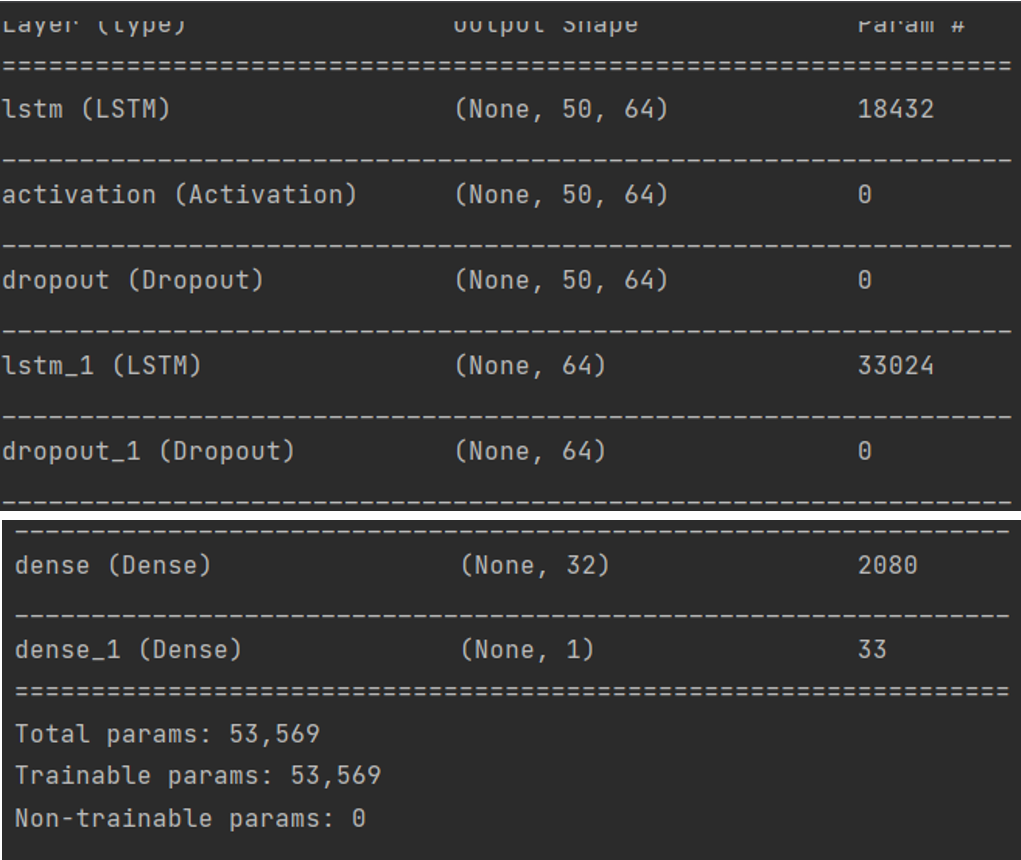
\includegraphics[width=0.5\textwidth]{images/FGNB.png}
  \caption{自定义多层LSTM模型} 
\end{figure}

我们构建模型的特色是选择了一个学习率观察器:\lstinline{lrate = ReduceLROnPlateau}
其参数是:\lstinline{monitor='val_loss', min_lr=0.00001, patience=patience,factor=0.5}。随后就可以拟合网络了。完整代码见下方:

\begin{lstlisting}[language=Python]
import math
from keras.losses import mean_squared_error
from keras.callbacks import ReduceLROnPlateau
from keras.optimizer_v2.adam import Adam
from matplotlib import pyplot as plt
from tensorflow.keras.layers import SimpleRNN
from tensorflow.keras.layers import Dense
from tensorflow.keras.models import Sequential
from keras.layers import Dropout, LSTM, Activation

# 搭建lstm网络模型,activation="RELU"
model = Sequential()
model.add(LSTM(units=64, return_sequences=True, input_shape=(train_X.shape[1], train_X.shape[2])))
model.add(Activation("relu"))
model.add(Dropout(0.2))
model.add(LSTM(units=64, return_sequences=False))
model.add(Dropout(0.2))
# model.add(SimpleRNN(units=64, return_sequences=False))
# model.add(Dropout(0.5))
model.add(Dense(32))
# 原本是model.add(Dense(32))
model.add(Dense(1))

model.compile(loss='mean_squared_error', optimizer=Adam(learning_rate=learning_rate),metrics=['accuracy'])
model.summary()


lrate = ReduceLROnPlateau(monitor= 'val_loss',min_lr=0.00001,patience=patience,factor=0.5)
# 拟合网络,batch_size默认32
history = model.fit(train_X,
                    train_y,
                    epochs = epochs,
                    batch_size=batch_size,
                    validation_data=(test_X, test_y),
                    callbacks=lrate,
                    verbose=1,
                    shuffle=True)
# 保存模型
model.save('results/LSTM.h5')
我们用plt可以简单画出训练图像。
	# 绘制历史数据
plt.plot(history.history['loss'], label='train')
plt.plot(history.history['val_loss'], label='val')
plt.legend()
plt.show()
# 模型评估
score = model.evaluate(test_X, test_y, verbose=0)
print(score)
# 观察结果
\end{lstlisting}

\begin{figure}[H]
  \centering
  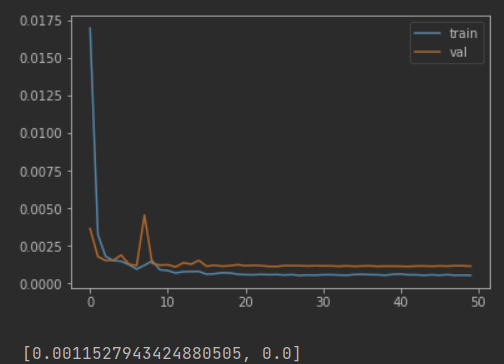
\includegraphics[width=0.5\textwidth]{images/FGN.png}
  \caption{LSTM模型训练} 
\end{figure}

我们能看到它的测试集得分值非常的小,证明我们的模型还是较为精确的。接下来加载模型进行预测:

\begin{lstlisting}[language=Python]
from tensorflow.keras.models import load_model
# 加载模型调入测试集尝试一下
model_path = 'results/LSTM.h5'
model = load_model(model_path)

predicted_data = model.predict(test_X)
print(test_y.shape)
print(predicted_data.shape)
print(predicted_data[:,0].shape)
# predicted_data
# (309,)
# (309, 1)
# (309,)
fig = plt.figure(facecolor='white')
ax = fig.add_subplot(211)
ax.plot(test_y, label='True Data')
ax.plot(predicted_data[:,0], label='Prediction_1')
ax.legend()
plt.show()
\end{lstlisting}

\begin{figure}[H]
  \centering
  \includegraphics[width=0.5\textwidth]{images/FGNN.png}
  \caption{LSTM验证集拟合} 
\end{figure}

可以看到我们的预测值(黄色)和真实值(蓝色)十分贴近,这无疑给了我们小组工作结果极大的肯定。下面给出我们本地的预测结果:

\begin{lstlisting}[language=Python]
pre_1_dim = predicted_data[:,0]
rmse = math.sqrt(mean_squared_error(test_y,pre_1_dim))
print("模型的RMSE:{}".format(round(rmse,3)))
\end{lstlisting}

输出:
模型的RMSE:0.034


可以看到这个值还是非常小的,令人精神一振。下面我们读取一下训练好的模型,来进行对平台测试集的预测。还是如同前面一样的数据处理方法,这里我们把它编进一个predict函数中。6、7列温度数据依旧采用加和平均方法。

\begin{lstlisting}[language=Python]
# 读取数据输出结果
def predict(sequence):
    # 数据处理
    sequence = sequence.astype('float64')
    sequence = np.expand_dims(sequence, 0).repeat(1, axis=0)
    # print(sequence.shape)
    pre_t = model.predict(sequence)
    pre_t = np.float64(pre_t)
    return pre_t

a=np.loadtxt('train_input.csv',dtype=np.float64)
a[5] =(a[6]+a[5])/2
a = np.delete(a,6,axis=1)
b=np.loadtxt('output.txt',dtype=np.float64)
b = b[:,np.newaxis]

c=np.loadtxt('test_input.csv',dtype=np.float64)
c[5] = (c[5]+c[6])/2
c = np.delete(c,6,axis=1)
d=np.ones([798,1], dtype = np.float64)

values=np.concatenate((a,b),axis=1)
values2=np.concatenate((c,d),axis=1)
values = values[-number1:,:]
print(values.shape)
print(values2.shape)
\end{lstlisting}

输出为:
(50, 7) 
(798, 7)

这里我们输出一共有7列,但是实际上只要取用第一列就可以了。最后,我们使用循环来进行递归预测。一共798个数据因此要循环798次,每个值都是用前100个数的值进行预测的,滑动窗口以此类推。同时还要注意其中的相关数据维度变换。当发现数据维度我们不清楚时,就可以在每一步输出出来进行观察和代码调试。

\begin{lstlisting}[language=Python]
for i in range(798):
    # print(predict(values))
    pre=predict(values)
    d[i] = pre
    values = np.delete(values, 0, axis = 0)
    values2[i,6]=d[i]
    e = values2[i]
    e = e[np.newaxis,:]
    #print(e.shape)
    values=np.concatenate((values,e),axis=0)
    #print(values.shape)
data = pd.DataFrame(values2)
writer = pd.ExcelWriter('results/TESTLSTM.xlsx')
data.to_excel(writer, 'page_1', float_format='%.32f')		
# ‘page_1’是写入excel的sheet名
writer.save()
writer.close()
\end{lstlisting}

自此,我们就实现了所有的预测内容,实践证明,递归LSTM有了良好的效果。
但是我们还是要来研究一下下面这幅图:

\begin{figure}[H]
  \centering
  \includegraphics[width=0.5\textwidth]{images/FGNNN.png}
  \caption{LSTM测试集拟合} 
\end{figure}

能发现几个问题:

\begin{enumerate}
  \item 递归LSTM的预测值会在某些高点过分放大特征,导致这些点的值偏高,会放大误差。
  \item LSTM的预测有滞后趋势。
  \item 递归LSTM的数据预测是上翘的。
\end{enumerate}

为了解决这些问题,首先我们选择了非递归LSTM的结果和递归LSTM的结果进行比较,在一些最高点附近我们对其进行松弛平均,即在预测值设置惯性值调节高点值不要太高。

其次我们对时间步长进行选择,尽可能减少LSTM上翘趋势。

最后我们让整体预测结果采取梯度的下沉,以减小数据整体的上翘趋势。因此我们就得到了下面的图进行对比。


\begin{figure}[H]
  \centering
  \includegraphics[width=0.5\textwidth]{images/FGNNNN.png}
  \caption{LSTM测试集拟合(处理前后对比)} 
\end{figure}

实践证明,这些方法让我们预测结果更加精准。在平台上测试时也取得了第一名的成绩。

\begin{figure}[H]
  \centering
  \includegraphics[width=0.5\textwidth]{images/SSSS.png}
  \caption{测试平台成绩(第一名)} 
\end{figure}


\begin{figure}[H]
  \centering
  \includegraphics[width=0.5\textwidth]{images/SSSSS.png}
  \caption{测试平台成绩记录} 
\end{figure}

\section{小组分工与感想}

\subsection{分工}


\subsubsection{王子非}
OLS、PLS、随机森林、SVM、LSTM、递归LSTM等模型搭建以及优化。

\subsubsection{刘可佳}
数据预处理以及多元线性回归、逻辑回归、BP神经网络、LSTM、递归LSTM等模型搭建。

\subsubsection{李浩东}
数据分析以及CNN、RL、DNN、CAE等模型搭建以及优化。

\subsection{感想}

\subsubsection{王子非}

我在这次的数据建模课程中完成了如下任务:

\begin{enumerate}
  \item 开题展示汇报、中期展示汇报、结题展示汇报
  \item ols、pls、svr、随机森林模型的搭建
  \item RNN、简单LSTM、递归LSTM代码的编写和完善
  \item RNN、LSTM模型的参数调整和优化
  \item 背景知识、ols、pls、svr、随机森林、lstm部分的报告撰写
\end{enumerate}

通过本课程的学习和实践,我加深了对数据驱动、数据建模以及数据应用的认识,
并使用数据方法来解决了生活中的实际问题。在完成小组作业的过程中,
我对各种算法逐渐熟悉,在模型编写和参数调整的过程中逐渐得到了关于机器学习和深度学习的实践体会。
我还对时序数据的处理有了从浅显到深刻的理解,面对参数调整时也逐渐得心应手,同时还强化了我对模型的认识和编写能力。
总之,这次课程让我收获很多,感谢老师和同学们对我的帮助!

\subsubsection{刘可佳}
通过本次课程实践,我对各种预测模型的搭建还有数据预处理方法有了进一步了解。LSTM相比其他模型在本问题的解决上有较大的优势,模型本身适合时序预测,而且能很简单地得到较好效果。建模过程初始,我写的几个模型的效果总是不尽人意,其中表现最好的竟然是线性回归,这让我很挫败。在想出递归LSTM这个思路后,我立马着手搭建,在经过队友的调参之后一下子就取得了很好的成果。本课程激发了我对数据驱动建模的兴趣,希望我在今后的学习中能够对该部分内容有进一步的学习并取得更大的收获。

\subsubsection{李浩东}

\begin{enumerate}
  \item 对于数据预处理、模型搭建等不能想当然,比如数据量越多信息就越全面,模型也会得到越优秀的结果,是不一定的,引入了噪声模型的泛化能力会严重下降
  。所以一定要实事求是,用事实说话。
  \item 模型越复杂不代表更表现好,要使用最合适的,要在充分的数据分析的基础上,结合各种组合以及数学上的变换与滤波,提升数据质量,数据质量是模型取得较为优秀的泛化性能的关键。
  \item 神经网络等模型的可解释性并不是很好,在时间充裕的情况下一定要多多尝试,思考数据本身的特征与性质,以此为出发点进行充分尝试。
  \item 信息越多并不意味着效果越好,噪声的危害很大,数据质量很关键,一定要保证有效数据占据绝对主导,噪声一定要平均。
\end{enumerate}

\section{APPENDIX: Source Code}

我们将代码放在了Github上:\href{https://github.com/LeBronLiHD/ZJU2021_Data-driven_Modeling_Application}{Github Link}

% \end{twocolumn}
\nocite{*}
\bibliography{books}
\end{multicols}
\end{document}
%%%%%%%%%%%%%%%%%%%%%%%%%%%%%%%%%%%%%%%%%%%%%%%%%%%%%%%%%%%%%%%%%%%%%%%%%%%%%%%%%%%%%%%%%%%%%%%%%%%%%%%%%%%%%%%%%%%%%%%%%%%%%%%%%%%%%%%%%%%%%%%%%%%%%%%%%%%%%%%%%%%%%%%%%%%%%%%%%%%%%%%%%%%%%%%%%%%%%%
\begin{description}
 \item[First] \hfill \\
 The first item
 \item[Second] \hfill \\
 The second item
 \item[Third] \hfill \\
 The third etc \ldots
\end{description}

\begin{equation}
(a+3b)^{n} = \sum_{k=0}^{n} C_{n}^{k} a^{n-k} (3b)^k\label{eq:binom}
\end{equation}

\begin{lstlisting}
\usepackage[UTF8,scheme=plain]{ctex}
\end{lstlisting}

\begin{enumerate}
\item 软件功能质量:
\item 软件结构质量:
\end{enumerate}

\begin{quote}
指能指挥计算机工作的程序、程序运行时所需要的数据以及与这些程序和数据有关的文档。
\end{quote}

\lstinline{}

\begin{itemize}
\item 程序是按事先设计的功能和性能要求执行的指令序列;
\item 数据是使程序能正常操纵信息的数据结构;
\item 文档是与程序开发,维护和使用有关的图文材料。
\end{itemize}

在引出本文的研究方向(软件复杂度与bug对软件质量的影响)之前,笔者首先对整体上软件的部分概念做简要陈述。

\subsection{软件的定义与内涵}
在简要浏览所给数书目后,笔者决定选择Shari Lawrence Pfleeger的著作《Software Engineering , Theory and Practice》作为本文的主要参考书目\supercite{test}。软件作为现代社会的重要部分,是一个值得研究的对象,据\href{https://en.wikipedia.org/}{维基百科(Wikipedia)}\supercite{tuantuan},软件的定义为:
\begin{quote}
\textbf{Software} is a collection of data or computer instructions that tell the computer how to work. This is in contrast to physical hardware, from which the system is built and actually performs the work.
\end{quote}
此外,课程《软件技术基础》\footnote{之后简称为:《软基》}中关于软件系统(Software)的定义是:
\begin{quote}
指能指挥计算机工作的程序、程序运行时所需要的数据以及与这些程序和数据有关的文档。
\end{quote}
定义中关于名词“程序”、“数据”、“文档”的解释为:
\begin{itemize}
\item 程序是按事先设计的功能和性能要求执行的指令序列;
\item 数据是使程序能正常操纵信息的数据结构;
\item 文档是与程序开发,维护和使用有关的图文材料。
\end{itemize}
目前关于软件的看法,往往仁者见仁,智者见智\dots

\subsection{软件与硬件的关系}
在了解过部分学者关于软件定义与内涵的看法后,笔者发现,很多学者将软件(Software)与硬件(Hardware)分开看待,正如Yale N. Patt\footnote{Yale N. Patt: Professor of Electrical and Computer Engineering,
Ernest Cockrell, Jr. Centennial Chair in Engineering, and
University Distinguished Teaching Professor,
The University of Texas at Austin}所说:
\begin{quote}
It is as if there were a big wall between the hardware (the computer and how it actually works) and the software (the programs  that  direct  the computer's  bidding), and that one should be content to remain on one side of that wall or the other.  
\end{quote}
强调软件基于硬件实现功能,却经常忽略软件与硬件之间密不可分的关联,笔者认为,只有精通软件与硬件之间的关联,才可以设计出优秀的计算机系统,Yale N. Patt在其著作《Introducion to Computing Systems (2nd Edition)》\supercite{test}中讲到:
\begin{quote}
As you approach your study and practice of computing, we urge you to take the opposite approach—that  hardware and software are names for components of two parts of a computing system that work best when they are designed by someone who took into account the capabilities and limitations of both. 
\end{quote}
真正理解计算机程序需求的硬件设计者才可以\dots

\section{软件质量}
\subsection{软件质量的定义}
软件质量可以大致分为两个方面:
\begin{enumerate}
\item 软件功能质量:基于功能需求或规格反映了其与给定设计的符合性。
\item 软件结构质量:是指软件满足需要交付的功能外的要求的优劣性,例如健壮性或可维护性。
\end{enumerate}

\subsection{软件质量的评估}
ISO9126软件质量模型(图一)是评价软件质量的国际标准,由6个特性和27个子特性组成\supercite{tuantuan}。对于大部分的软件,都可以考虑从这几个方面着手进行测评。
% \begin{figure}[htbp]
\begin{figure}[H]
  \centering
  \includegraphics[width=0.5\textwidth]{images/SQ.png}
  \caption{ISO 9126 软件质量模型} 
\end{figure}
在我国,现行的软件质量评估标准是由中华人民共和国国家质量监督检验检疫总局和中国国家标准化管理委员会共同编撰《软件质量量化评价规范\supercite{test}(Specification for the quantitative evaluation of software quality)》。

\subsection{软件质量的进一步分析}
笔者认为,软件质量可以有两个视角\dots

\begin{table*}
  \centering
  \caption{Table of students.}
  \begin{tabular*}{\hsize}{@{}@{\extracolsep{\fill}}ccc@{}}
  \hline
  Name & Age & Gender  \\ \hline
  Cat & 3  & Girl  \\ \hline
  Dog & 5 & Boy \\
  \hline
  \end{tabular*}
  \label{table:stu}
  \end{table*}

软件质量是贯穿到软件的整个生命周期中(图二),从问题定义、可行性研究、需求分析、系统设计、详细设计、编码、测试、运行与维护。一旦在某一步骤出现疏漏,就会导致几乎所有子步骤的错误(图三)。
\begin{figure}[H]
  \centering
  \includegraphics[width=0.5\textwidth]{images/LLCC.png}
  \caption{软件的生命周期} 
\end{figure}
\begin{figure}[H]
  \centering
  \includegraphics[width=0.5\textwidth]{images/358.png}
  \caption{错误的传递} 
\end{figure}
软件质量非常重要,特别是对于商业软件和系统软件(例如Microsoft Office,Microsoft Windows和Linux)\dots

\section{软件复杂度}
著名计算机研究学者Brian Kernighan\footnote{Brian Wilson Kernighan (born January 1, 1942): a Canadian computer scientist.}在其著作中指出:
\begin{quote}
Controlling complexity is the essence of computer programming.
\end{quote}
软件复杂度是软件的重要衡量指标,与软件质量的联系十分密切,下面本文将给出关于软件复杂度的论述。

\subsection{软件复杂度的定义}
软件复杂度是软件的重要属性\supercite{tuantuan}。复杂意味着\dots

\subsection{软件复杂度的分析}
\subsubsection{软件复杂度的不利影响}
软件复杂度是灵活性的敌人。软件复杂度让我们陷入不可预期的结果\dots

\subsubsection{软件复杂度的原因}
软件复杂性的产生原因十分复杂,对于软件的生命周期而言,主要有以下几点:
\begin{enumerate}
\item 需求复杂、应用要求高;
\item 开发环境复杂;
\item 软件应用框架、结构及模型复杂;
\item 软件开发过程复杂;
\item 涉及人的智力和管理复杂;
\item 项目设计与验证复杂。
\end{enumerate}

如下图所示:
\begin{figure}[H]
  \centering
  \includegraphics[width=0.5\textwidth]{images/SC.png}
  \caption{软件的复杂度} 
\end{figure}

笔者认为,现实世界本身就是复杂的。这个是本质复杂度。

\section{软件bug}
软件bug是我们所不期望遇见的,不论是软件的开发者与使用者,正如下面这段话所说:
\begin{quote}
Software will change the world, but bug will destroy it.
\end{quote}
软件bug会造成很多不同程度上的错误,其中不乏十分严重的错误,比如:
\begin{quote}
1963年,美国飞往火星的火箭爆炸,损失大约\$10 million。原因为: \lstinline{FORTRAN}循环\lstinline{DO  5  I = 1,  3}误写为\lstinline{DO  5  I = 1.3}。
\end{quote}
软件bug同样也是衡量软件质量评估的重要参考因素。下面本文将对软件bug进行论述。
\subsection{软件bug的定义}
软件bug是指计算机程序或系统中的错误\dots

\subsection{软件bug的修复}
下面,本文将从软件bug的修复成本以及软件生命周期不同阶段如何减少bug的注意事项两方面论述软件bug的修复相关内容。

\subsubsection{软件bug的修复成本}
软件bug的成本有这样一条规律:发现的越晚,修复的成本越高,比如:
\begin{quote}
软件Aspen的运行与维护:MIT 30教授为首,联合50家公司,历时五年(1976-1981)开发运行,总共耗资600万美元。
\end{quote}
在最终交付给客户的产品或者服务时发现的bug, 比引入阶段发现的bug,其影响和修复成本要高出数倍(如图五),这一点类似问题汽车的召回。
\begin{figure}[H]
  \centering
  \includegraphics[width=0.5\textwidth]{images/COST.png}
  \caption{软件bug的修复成本与发现时间的关系} 
\end{figure}
此外,在软件生命周期的不同阶段,引入的bug的数量往往是不一样的,不难理解,大约85\%的bug是在软件开发的编码时期被引入的(如图六)。
\begin{figure}[H]
  \centering
  \includegraphics[width=0.5\textwidth]{images/507.png}
  \caption{不同阶段bug的数量} 
\end{figure}
而且,不同的阶段我们能够发现的bug的数量是不一样的\dots

\subsubsection{软件bug的修复成本}
下面本文将从不同的阶段对bug的修复进行论述。
\begin{itemize}
\item 需求探索时期

这个阶段需要软件开发团队\dots

对于一个全新的产品,DesignThinking\dots

\item 软件设计时期

设计是承上启下的步骤\dots

\item 软件编码阶段

这个阶段bug引入最多\dots

\begin{enumerate}
\item Pair Programming\footnote{Pair Programming下,同一个算法、同一段代码或同一组测试、与两位程序员各自独立工作相比,往往只需花费大约一半的时间就能编写出质量更高的代码。}
\item Code Review\footnote{Code Review:代码评审也称代码复查,是指通过阅读代码来检查源代码与编码标准的符合性以及代码质量的活动。}
\item  Code Inspect\footnote{Code Inspect:IDE的静态分析。}
\item SCS(Static Code Scan)\footnote{Static Code Scan:在软件工程中,程序员在写好源代码后,无需经过编译器编译,而直接使用一些扫描工具对其进行扫描,找出代码当中存在的一些安全漏洞的解决方案。}
\item Unittest\footnote{Unittest是一种完整的测试结构,支持自动化测试的执行,对测试用例集进行组织,并且提供了丰富的断言方法,最后生成测试报告。}
\item TDD(Test-Driven Development)\footnote{TDD是一种软件工程实践,要求在应该验证的代码之前编写单元测试。}(如图七)
\end{enumerate}

\begin{figure}[H]
  \centering
  \includegraphics[width=0.5\textwidth]{images/TDD.png}
  \caption{TDD Cycle} 
\end{figure}

\item 软件的运维阶段

传统软件发布是一个安装包\dots
\begin{enumerate}
\item 运行环境的监控
\item 应用程序的黑盒监控
\item log的信息
\end{enumerate}
其中log里面的warning 和error一定要去留意\dots
\end{itemize}

\section{结语}
结语。
